\documentclass[11pt,letterpaper]{article}
\usepackage[T1]{fontenc}
\usepackage[utf8]{inputenc}
\usepackage{amsthm}
\usepackage{newtxtext,newtxmath}
\usepackage[margin=1in,headheight=15pt]{geometry}
\usepackage{microtype,mathtools,booktabs,longtable,array,enumitem}
\usepackage[dvipsnames]{xcolor}
\usepackage{fancyhdr,titlesec}
\usepackage[most]{tcolorbox}
\usepackage{xurl}
\usepackage{graphicx,listings}
\usepackage[colorlinks=true,linkcolor=MidnightBlue,citecolor=MidnightBlue,urlcolor=MidnightBlue]{hyperref}
\hypersetup{pdftitle={Countable Information, Uncountably Many Boxes},pdfauthor={Research note prepared for Vladimir Reshetnikov},pdfsubject={Measurable box games, decision trees, enumeration, and asymptotics}}
\definecolor{ink}{HTML}{17344A}
\definecolor{accent}{HTML}{28797B}
\definecolor{paperblue}{HTML}{F2F6F8}
\titleformat{\section}{\large\bfseries\color{ink}}{\thesection}{0.65em}{}
\titleformat{\subsection}{\normalsize\bfseries\color{ink}}{\thesubsection}{0.65em}{}
\pagestyle{fancy}
\fancyhf{}
\fancyhead[L]{\small\itshape Countable Information, Uncountably Many Boxes}
\fancyhead[R]{\small Research note}
\fancyfoot[C]{\thepage}
\renewcommand{\headrulewidth}{0.3pt}
\setlength{\parskip}{0.35em}
\setlength{\parindent}{1.2em}
\setlist{itemsep=0.2em,topsep=0.3em}
\setcounter{tocdepth}{1}
\newtheorem{theorem}{Theorem}[section]
\newtheorem{lemma}[theorem]{Lemma}
\newtheorem{proposition}[theorem]{Proposition}
\newtheorem{corollary}[theorem]{Corollary}
\theoremstyle{definition}
\newtheorem{definition}[theorem]{Definition}
\newtheorem{example}[theorem]{Example}
\newtheorem{remark}[theorem]{Remark}
\newcommand{\N}{\mathbb N}
\newcommand{\R}{\mathbb R}
\newcommand{\E}{\mathbb E}
\newcommand{\Prb}{\mathbb P}
\newcommand{\ind}{\mathbf 1}
\newcommand{\Sig}{\Sigma}
\newcommand{\supp}{\operatorname{supp}}
\newcommand{\sg}{\sigma}
\newcommand{\floor}[1]{\left\lfloor #1\right\rfloor}
\newcommand{\restr}{\mathbin{\upharpoonright}}
\newcommand{\qset}{\{0,\ldots,q-1\}}
\newcommand{\repo}{\texttt{ProveIt}}
\newcommand{\commit}{\nolinkurl{6fef5383b126be343cccc9baf47081ef37ab5afe}}
% Part II (batch 90, manuscript 02) macros and environments
\newcommand{\F}{\mathbb F}
\newcommand{\xor}{\mathbin{\oplus}}
\newcommand{\as}{\text{a.s.}}
\newcommand{\FIN}{\operatorname{FIN}}
\newtheorem{question}[theorem]{Research question}
\definecolor{muted}{HTML}{596575}
\lstset{basicstyle=\small\ttfamily,breaklines=true,columns=fullflexible,
  frame=single,rulecolor=\color{muted},showstringspaces=false}
\newtcolorbox{resultbox}{colback=paperblue,colframe=accent,boxrule=0.6pt,arc=1mm,left=9pt,right=9pt,top=7pt,bottom=7pt,breakable}
% [write] Notes added when the manuscript joined ProveIt's research-report
% collection (batch 87, 3 October 2026) are set in this environment.
\newenvironment{writenote}[1][]{\par\smallskip\begingroup\small
 \noindent\textbf{[write]}\if\relax\detokenize{#1}\relax\else~\textbf{#1.}\fi\ }%
 {\par\endgroup\smallskip}
\begin{document}
\hypersetup{pageanchor=false}
\begin{titlepage}
\setlength{\parindent}{0pt}
\vspace*{0.15in}
{\color{accent}\sffamily\bfseries RESEARCH AT THE INTERSECTION OF SET THEORY AND COMPUTATION\par}
\vspace{0.20in}
{\fontsize{29}{33}\selectfont\bfseries\color{ink} Countable Information,\\[4pt] Uncountably Many Boxes\par}
\vspace{0.2in}
{\Large Sharp measurable prediction bounds, exact decision-tree enumeration, and an all-orders asymptotic expansion\par}
\vspace{0.25in}
{\large Prepared for Vladimir Reshetnikov\par}
{October 3, 2026\par}
\vspace{0.20in}
\begin{abstract}
We study the distinction between choosing an unread coordinate and assigning a measurable event to a correct prediction. For a nonempty standard Borel set of boxes, a finite alphabet of size $q$, and $m$ deterministic players whose output maps are measurable for the cylinder $\sigma$-algebra, we prove that the optimal guaranteed number of correct guesses is exactly $\floor{m/q}$. The proof does not assume that success events are measurable. A simultaneous measure-extension construction supplies fair success probabilities for any countable collection of such players. Conversely, measurability of a blind player's success event forces its target range to be countable, pointwise or outside a cylinder-null set according to the chosen completion.

The finite problem leads to a separate structural result. Blind binary output maps correspond to labeled perfect matchings of the hypercube, whereas executable maps correspond precisely to recursively sliceable matchings. We derive an exact inclusion--exclusion recurrence for the latter, prove that the two classes first differ at four boxes, and establish
\[
 F_n=\frac{e^{\gamma 2^n}}{n}\left(1-\frac{3}{2n}+\frac{17}{4n^2}
 -\frac{12}{n^3}+O(n^{-4})\right),
\]
with a rational algorithm for every further asymptotic coefficient. We also prove an explicit doubly exponential upper bound on the fraction of blind maps that are executable. Finite checks, an oracle counterexample-extraction theorem, and a Busy Beaver obstruction connect the analysis to the certificate-oriented architecture of \repo.
\end{abstract}
\vfill
\begin{resultbox}
\textbf{Scope and status.} All stated theorems have proofs in this note. The finite computations were executed independently in Python. The infinite results have not been checked in Lean or Rocq, and historical priority is not established. The restricted measurable problem is settled here; Glazer's unrestricted question about what ZF proves is not settled here. Neither authorship nor endorsement by Elliot Glazer is implied.
\end{resultbox}
\smallskip
{\footnotesize\textbf{[write]} Filed in ProveIt's research-report collection as \texttt{ordinals-and-order-types/measurable-box-games} (batch~87, manuscript~02; label prefix \texttt{mbg:}). Provenance, the checks made at intake, and the notation table are in Sections~\ref{mbg:sec:provenance} and~\ref{mbg:sec:notation}.\par}
\end{titlepage}
\hypersetup{pageanchor=true}
{\footnotesize\noindent\textbf{[write]} Since 4 October 2026 the report has two Parts: Part~\ref{mbg:hat:part} (from Section~\ref{mbg:hat:sec:introduction}; batch~90, labels \texttt{mbg:hat:}) treats surplus in hat guessing and settles Q9 for one family; Part~\ref{mbg:part:one}'s numbering is unchanged.\par}
\tableofcontents
\newpage

\part{Sharp measurable prediction bounds, exact decision-tree enumeration, and an all-orders asymptotic expansion}
\label{mbg:part:one}

\section{Research question and contribution map}

Glazer studies prediction games in which players inspect boxes and then guess an unopened value. In Section 5 of \cite{GlazerBox}, he asks whether ZF proves that three players with continuum many binary boxes can guarantee at least two correct guesses. His work on weak choice principles \cite{GlazerChoice} and the finite and infinite puzzles described in his research profile \cite{GlazerProfile} make regularity, executability, and explicit axiomatic boundaries natural questions to investigate.

The relevant \repo\ materials are its Busy Beaver machine interface, finite-list coding in arithmetic, and explicit first-order set-theoretic developments \cite{ProveIt,BusyBeaver,ListCoding,Closure}. Rather than importing an unverified mathematical claim from those projects, we use their architecture: distinguish a semantic statement from an executable certificate, and distinguish both from the theorem that validates the certificate. The repository snapshot used throughout is \commit.

The central issue is not a numerical estimate. On an uncountable product, the following statements are different:
\begin{enumerate}[label=(\roman*)]
\item the rule selecting a box and a guess is measurable;
\item the event that the selected box contains the guess is measurable;
\item the rule can actually be implemented without inspecting its final target.
\end{enumerate}
None of these distinctions can safely be suppressed. We obtain two complementary lines of results.

\subsection{The continuum line}
Theorem~\ref{mbg:thm:minimax} gives the exact measurable-output minimax value, including the three-player binary case. Theorem~\ref{mbg:thm:fresh} constructs a simultaneous fair extension of the product probability for countably many players. Theorem~\ref{mbg:thm:collapse} shows that measurable success is a much stronger restriction on the range of targets than measurable output. The diagonal example in Section~\ref{mbg:sec:diagonal} makes the difference explicit: its output rule is continuous, but its success event has inner measure zero and outer measure one. We classify every extension obtained by adjoining that event.

\subsection{The finite line}
Theorem~\ref{mbg:thm:slice} characterizes executable binary output maps by a recursive property of hypercube matchings. The sequence $F_n$ counting the underlying executable matchings begins
\[
1,\ 2,\ 9,\ 232,\ 206065,\ 212181312096,\ldots.
\]
It is \emph{not} the sequence of all perfect matchings, OEIS A005271 \cite{OEIS}; that sequence already differs at $n=4$. We prove an exact recurrence, a full asymptotic expansion, and an explicit rarity bound. These results are not asserted to be absent from the literature or the OEIS: exact-sequence searches did not yield a usable classification during this investigation.

\subsection{What is, and is not, claimed as a contribution}
The countable-support lemma, finite-coordinate averaging, Radon--Nikodym theorem, compactness of a finite-alphabet sequence space, and halting-time diagonalization are standard ingredients. The contribution developed here is their precise application to the output/success distinction, together with the decision-tree classification, enumeration, asymptotic calculation, and executable finite checks. The measure-extension classification is a special-case application of the classical theory represented by \L o\'s and Marczewski \cite{LosMarczewski}, not a claim to have invented measure extension.

These statements constitute a research note with complete proofs and testable finite consequences. They are not presented as a verified historical breakthrough or as a resolution of an unrestricted choiceless-set-theory problem.

\subsection{Provenance and place in the collection}
\label{mbg:sec:provenance}

\begin{writenote}[Added 3 October 2026, batch~87]
This report is a single manuscript, printed in full: manuscript~02 of batch~87 of ProveIt's incoming-reports intake, delivered as the archive \texttt{glazer\_\allowbreak box\_\allowbreak games\_\allowbreak research.zip} (inner directory \texttt{glazer\_\allowbreak box\_\allowbreak games/}, main file \texttt{article.tex}, a 24-page US Letter PDF) in the arrival commit \texttt{fa0a0576e}, and placed in commit \texttt{d151b39ca} in the research-report collection as \texttt{ordinals-and-order-types/\allowbreak measurable-box-games}. The author line reads ``Prepared for Vladimir Reshetnikov'' and carries no AI wording; like the other deliveries of the intake, the report is AI-assisted, unrefereed and not formalized. Its five sister manuscripts of batch~87 concern Glazer's \emph{other} question paper, \emph{A Topological Tennenbaum Theorem} (arXiv:2311.13699), and became Parts~VI--IX of the surreal-collection report \nolinkurl{Algebra/SurrealNumbers/docs/foundations-and-computation/polish-models-of-omnific-arithmetic}; this manuscript shares no theorem, question or notation with them. Being a single source, the report needed no merge choices. The write prefixed all 61 delivered labels with \texttt{mbg:} and updated every reference; added the four labels \texttt{mbg:sec:provenance}, \texttt{mbg:sec:notation}, \texttt{mbg:app:ledger} and \texttt{mbg:app:audit}; added these dated \textbf{[write]} notes, the title-page line, the \texttt{pageanchor} switch around the title page (a delivered build gave a duplicate \texttt{page.1} destination) and a dated addition to the bibliography entry~\cite{GlazerBox}. No statement, proof, number or non-claim of the manuscript was changed.

\emph{Pin and repository claims.} The pin \commit\ (\texttt{6fef5383b}, quoted throughout) is the ProveIt commit the manuscript was written against; it is an ancestor of the placement. The three repository files it read, \nolinkurl{Computability/BusyBeaver/Lean/BusyBeaver/Core.lean}, \nolinkurl{Logic/PeanoArithmetic/ListCoding/README.md} and \nolinkurl{SetTheory/ClosureAxiomatization/README.md}, were byte-identical at the pin and at the write (blobs \texttt{4961655e}, \texttt{74164ac6}, \texttt{fb0ab511}), and the descriptions of them in Sections~\ref{mbg:sec:computability} and~\ref{mbg:sec:foundations} are accurate: the Busy Beaver core's opening comment separates the blank-tape machines and the maximum property of the score function from a separately stated compiler fact; the list-coding README documents validity guards, unique decoding and round trips; the closure-axiomatization README separates its semantic directions from the deductive-equivalence layer. At placement the intake searched the whole tracked tree for box, hat, guessing and prediction games, for \texttt{2211.10474} and for A005271, and found nothing: no report or formal project in ProveIt treats this question, and the report continues no repository material. Its place in the collection confers no formal status; no statement of it is formalized in Lean or Rocq.

\emph{Glazer's paper.} The arXiv record of~\cite{GlazerBox}, read on 3 October 2026, lists a single version, v1 of 15 November 2022 (6 pages; math.LO, math.CO; DOI \nolinkurl{10.48550/arXiv.2211.10474}); the date line ``January 9, 2023'' that the manuscript's ``inspected PDF'' carries is printed in arXiv's PDF of that same v1, not a revision. The question of Section~5 (``More box games'') of that paper reads ``Does ZF prove that $G([3],\mathbb R,\{0,1\})$ is winnable?'', where winning means that at most one of the three players guesses wrong; it is Research question~Q1 of Section~\ref{mbg:sec:questions}. \textbf{It is not the ``Glazer's Question~1'' of the surreal report above}, which is Question~1 of the Topological Tennenbaum paper, about the reverse-mathematical strength of Glazer's Theorem~2 there.

\emph{Review in the Hilbert's-tenth research tree.} Before placement, another session reviewed all six batch-87 archives at their arrival revision (commit \texttt{f15962acd}): \nolinkurl{Computability/HilbertTenthProblem/Papers/research-wip/native-stream-queue/review_baire_polish_arithmetic_intake.md}, with an independent cross-reading in \nolinkurl{review_baire_polish_arithmetic_intake_independent.md} beside it and a receipt in \nolinkurl{review_baire_polish_arithmetic_intake.json}. For this manuscript it read the delivered lines 64--73, 82--110, 386--428, 776--820 and 927--955 (the abstract; Section~1 through Section~1.3; Section~\ref{mbg:sec:finite} from its start through Lemma~\ref{mbg:lem:restriction}; Section~\ref{mbg:sec:computability}; the conclusion and the ledger of Appendix~\ref{mbg:app:ledger}). It confirms the statements as scoped here: legal finite binary decision trees correspond to recursively sliceable matchings and blind output tables need not be executable; the extraction of Theorem~\ref{mbg:thm:extract} is a partial procedure for which the totality and legality promise is essential; no computable horizon bound from program length exists, and the Busy Beaver comparison is conditional on an encoding and an additive-overhead compiler. It records that these results give no fixed-size Diophantine history certificate and no paid arithmetic schedule, so they leave the Hilbert's-tenth programme's 84-operation universal polynomial unchanged, and that the probability, matching-enumeration and asymptotic claims were \emph{not} reviewed there. Nothing in the review required a change of scope here.

\emph{OEIS, checked at intake.} On 3 October 2026 the intake searched the OEIS for $1,2,9,232,206065$, for $9,232,206065$ and for the ternary $2,21,33976$: none matches an entry. The entry A005271, ``Number of perfect matchings in $n$-cube'', begins $1,2,9,272,589185,16332454526976,\ldots$, agreeing with $M_1,\ldots,M_5$ of Section~\ref{mbg:sec:enumeration}. This is a check of the database on that date, not of the literature, so the manuscript's own reservation in Section~1.2 stands. Nothing was submitted to the OEIS, by the manuscript's author or by the intake; any submission is a human editor's decision after review. An independent program at intake reproduced $F_1,\ldots,F_6$, the ternary $F^{(3)}_1,\ldots,F^{(3)}_5$, $D_6$, the integer comparison of Theorem~\ref{mbg:thm:rarity}, the 232 sliceable and 40 nonsliceable matchings of $\mathcal Q_4$ by brute force, and the two decimal enclosures of $\gamma$.

\emph{Neighbouring reports.} None shares a theorem. The games of \nolinkurl{ordinals-and-order-types/games-on-ordinals/} are different objects: in \nolinkurl{open-query-membership-games} a Seeker asks open-set queries about a hidden point on a topological space (its transcripts and finite-budget certificates are adaptive query strategies, but nobody guesses an unread coordinate); \nolinkurl{point-separating-game-values} and \nolinkurl{ordinal-chomp-transition-at-two} concern point-separating games and ordinal Chomp. \nolinkurl{ordinals-and-order-types/non-baire-translation-invariant-ideal} is the nearest in spirit: it builds, in ZFC from a free ultrafilter, an ideal without the Baire property, the kind of choice-built irregular object whose absence Research question~Q2 asks about for the Baire-property version of Theorem~\ref{mbg:thm:minimax}.
\end{writenote}

\begin{writenote}[Added 4 October 2026, batch~90]
Since 4 October 2026 this report has two Parts. Part~\ref{mbg:part:one} is the batch-87 manuscript described in the preceding note, printed as before: its sections, statements, equations, labels and bibliography numbers are unchanged (checked against a build of the batch-87 text), so the preceding note's ``single manuscript, printed in full'' now describes Part~\ref{mbg:part:one}. Part~\ref{mbg:hat:part} is manuscript~02 of batch~90, \emph{No Universal Sublinear Bound for Measurable Hat Guessing}, pinned at commit \texttt{7c0f2d9f9}; its provenance is Section~\ref{mbg:hat:sec:provenance}. It treats Eldredge's infinite binary hat game, in which every player's target is its own hat, and answers the two growth questions of his Remark~6.8~\cite{hat:Eldredge}; its Corollary~\ref{mbg:hat:cor:finite-optimal} settles Research question~Q9 below for the parameters $(m,q,n)=(2a(2^r-1),2,2a(2^r-1))$ and the threshold $a2^r$ (see the note after the questions of Section~\ref{mbg:sec:questions}). The statement above that nothing in ProveIt treats box, hat, guessing or prediction games was true at the batch-87 placement; Part~\ref{mbg:hat:part} is now such material, and the batch-90 placement (commit \texttt{12076b2e8}) found no other. The neighbouring reports named above share no theorem with Part~\ref{mbg:hat:part} either.
\end{writenote}

\subsection{Notation used in this report}
\label{mbg:sec:notation}

\begin{writenote}[Added 3 October 2026, batch~87]
The manuscript reuses several letters with local meanings. None was renamed; this table fixes the readings, with the tempting false one where confusion is likely.
\begin{center}\small
\begin{tabular}{>{\raggedright\arraybackslash}p{0.17\textwidth}>{\raggedright\arraybackslash}p{0.74\textwidth}}
\toprule
Symbol & Meaning (and what it is not)\\
\midrule
$\gamma$ & the growth constant $\lim 2^{-n}\log F_n\approx0.438158$ of \eqref{mbg:eq:gamma}; \emph{not} Euler's constant $0.5772\ldots$\\
$F_n$, $M_n$ & sliceable (executable) matchings of $\mathcal Q_n$; all perfect matchings (A005271). They first differ at $n=4$ ($232<272$).\\
$B_n$, $L_n$ & blind and legal binary output maps, $2^{2^{n-1}}M_n$ and $2^{2^{n-1}}F_n$; $B_n$ has nothing to do with a Busy Beaver function\\
$\operatorname{BB}_{\rm time}$, $H$ & a program-length running-time Busy Beaver function and the maximal horizon (Section~\ref{mbg:sec:computability}); \emph{not} Rado's $n$-state score function formalized in \nolinkurl{Computability/BusyBeaver}. In Section~\ref{mbg:sec:information}, $H$ is entropy.\\
$I$ & the set of boxes; in Section~\ref{mbg:sec:information} also mutual information $I(Z;X_K)$\\
$\E$, $E_\tau$, $E$ & expectation; the success set of $\tau$; the diagonal success set of Section~\ref{mbg:sec:diagonal}\\
$C$ & a group of players sharing an external target (proof of Theorem~\ref{mbg:thm:minimax}); Cantor space $2^\N$ (Section~\ref{mbg:sec:diagonal}); the formal series $C(z)$ of \eqref{mbg:eq:Cformal}\\
$D$ & the integer score $D(u)$ (proof of Theorem~\ref{mbg:thm:minimax}); the count $D_6$ of \eqref{mbg:eq:D6}; an event in the proof of Theorem~\ref{mbg:thm:information}\\
$r$ & list size (Corollary~\ref{mbg:cor:lists}); the ratio $r_n=F_n/F_{n-1}^2$; the label $r=x\restr\N$ in Section~\ref{mbg:sec:diagonal}\\
$R$, $\R$ & the formal series $R(z)$ of \eqref{mbg:eq:Rformal}; the real line\\
$T$, $L$ & the replacement map $T(Y,U)$ (Theorem~\ref{mbg:thm:fresh}); the time and prefix-length bounds $T$, $L$ in the proof of Theorem~\ref{mbg:thm:extract} ($L$ is not $L_n$)\\
$Q$, $\mathcal Q_n$, $q$ & the alphabet $\{0,\ldots,q-1\}$; the cube graph; the alphabet size (not a $q$-series variable)\\
$\Sig_I$ & the cylinder $\sigma$-algebra, \emph{not} the Borel $\sigma$-algebra of the product topology and not its completion\\
Q1--Q12 & Research questions of Section~\ref{mbg:sec:questions}; Q1 is Glazer's box-game question, not the ``Question~1'' of his Topological Tennenbaum paper\\
\bottomrule
\end{tabular}
\end{center}
\end{writenote}

\section{Configurations, blindness, and measurable output}
\label{mbg:sec:model}

Fix $q\ge2$, put $Q=\qset$, and let $I$ be a nonempty set. A \emph{configuration} is a function $x:I\to Q$. Write
\[
 X_I=Q^I,\qquad
 \Sig_I=\sg\{x:x_i=a\mid i\in I,\ a\in Q\}.
\]
The probability measure $\mu_I$ on $\Sig_I$ is the product measure under which every fixed finite family of coordinates is independent and uniform on $Q$.

\begin{remark}[Which $\sigma$-algebra?]
The cylinder $\sigma$-algebra $\Sig_I$ is not, by definition, the full Borel $\sigma$-algebra of the uncountable product topology. Nor is it automatically its own completion. Every measurability assertion below names the relevant $\sigma$-algebra. This is essential, not a technical convention that can be changed without affecting the theorems.
\end{remark}

For $i\in I$ and $v\in Q$, let $x^{i\leftarrow v}$ denote the configuration obtained by replacing $x_i$ by $v$ and leaving all other coordinates unchanged.

\begin{definition}[Blind output map]
An output map is a total function
\[
 \tau=(b,a):X_I\longrightarrow I\times Q.
\]
It is \emph{blind} if, whenever $\tau(x)=(i,c)$,
\begin{equation}
 \tau(x^{i\leftarrow v})=(i,c)\quad\hbox{for every }v\in Q.
 \label{mbg:eq:blind}
\end{equation}
Its success set is
\[
 E_\tau=\{x:x_{b(x)}=a(x)\}.
\]
For a team $\tau_1,\ldots,\tau_m$, the score is
$S(x)=\sum_{p=1}^m\ind_{E_{\tau_p}}(x)$.
\end{definition}

Every total deterministic legal probing strategy induces a blind output map. Indeed, altering only the value of its ultimately unopened box changes none of the observations along the original run. Induction on the successive moves gives the same history and the same final output. This remains a necessary condition when a move reveals an entire set of boxes or histories are transfinite. We do not identify blindness with legal executability; Section~\ref{mbg:sec:finite} gives a finite counterexample to that identification.

From now on, for the continuum theorems, $I$ carries a standard Borel structure. Measurability of $\tau$ means measurability from $(X_I,\Sig_I)$ to $I\times Q$ with its product Borel structure. In particular, singleton targets, equality of two target maps, and membership in any countable set of targets are measurable.

\begin{definition}[Coordinate support]
A set $A\subseteq X_I$ is \emph{supported by} $J\subseteq I$ if membership in $A$ is unchanged when coordinates outside $J$ change. A function is supported by $J$ if two configurations agreeing on $J$ have the same function value.
\end{definition}

\begin{lemma}[Countable-coordinate dependence]
\label{mbg:lem:support}
Every member of $\Sig_I$ has a countable support. Every $\Sig_I$-measurable map to a countably separated measurable space has a countable support. Consequently a finite or countable family of measurable maps to standard Borel spaces has a common countable support.
\end{lemma}
\begin{proof}
The sets possessing a countable support form a $\sigma$-algebra: complements keep the same support, and a countable union is supported by the union of its chosen supports. This $\sigma$-algebra contains each coordinate cylinder, proving the first assertion.

For a measurable function $f$, choose a countable family $(C_k)$ of measurable sets separating points in its codomain. Choose a countable support $J_k$ for $f^{-1}(C_k)$ and put $J=\bigcup_kJ_k$. If $x\restr J=y\restr J$, then $f(x)$ and $f(y)$ belong to exactly the same $C_k$, hence are equal. A further countable union gives the last assertion.

The factorization is literal, not merely almost everywhere. Fix the symbol $0$ outside $J$ and let $s_J:Q^J\to Q^I$ be the corresponding section. Then $s_J$ is measurable, $f_J=f\circ s_J$ is measurable, and $f=f_J\circ\pi_J$.
\end{proof}

The lemma is proved here in the ordinary classical setting. The selection of countably many supports is among the steps that need a separate audit before attributing this proof to a weak choiceless base theory.

\section{The sharp measurable-output bound}
\label{mbg:sec:minimax}

\begin{theorem}[Exact minimax value]
\label{mbg:thm:minimax}
Let $I$ be a nonempty standard Borel space and let $m\ge1$. For every team of $m$ blind cylinder-measurable output maps there is a configuration $x$ such that
\begin{equation}
 S(x)\le\floor{m/q}.
 \label{mbg:eq:minimax}
\end{equation}
There is a legal team of constant output maps guaranteeing at least $\floor{m/q}$ correct guesses on every configuration. Thus the optimum worst-case score in the measurable-output class is exactly $\floor{m/q}$.
\end{theorem}

\begin{proof}
Choose a common countable support $J$ for the outputs. On $Q^J$ write the factored outputs as $(b_p(u),a_p(u))$. We separate targets inside $J$ from targets outside $J$.

For $i\in J$ and $c\in Q$, the measurable fiber
\[
 A_{p,i,c}=\{u:b_p(u)=i,\ a_p(u)=c\}
\]
is invariant under changing $u_i$, by blindness. A product integration in that one coordinate gives
\begin{equation}
 \mu_J(A_{p,i,c}\cap\{u:u_i=c\})=\frac1q\mu_J(A_{p,i,c}).
 \label{mbg:eq:fiberfair}
\end{equation}
Therefore the internal score
\[
 S_{\rm in}(u)=\sum_{\substack{1\le p\le m\\ b_p(u)\in J}}
                  \ind_{\{u_{b_p(u)}=a_p(u)\}}
\]
is measurable and satisfies
\begin{equation}
 \E S_{\rm in}=\frac1q\sum_{p=1}^m\mu_J(b_p\in J).
 \label{mbg:eq:inside}
\end{equation}

For each fixed $u$, group the remaining players according to their common target outside $J$. If $C$ is one such group, let
$n_{C,v}(u)=|\{p\in C:a_p(u)=v\}|$. Give the shared target the least symbol minimizing $n_{C,v}(u)$. Its contribution to the score is then
\[
 \min_{v\in Q}n_{C,v}(u)\le |C|/q.
\]
Define the integer-valued function
\[
 D(u)=S_{\rm in}(u)+\sum_C\min_{v\in Q}n_{C,v}(u).
\]
There are only finitely many players. The grouping is determined by finitely many measurable equality tests among their targets, so $D$ is measurable. From \eqref{mbg:eq:inside},
\[
 \E D\le\frac1q\sum_p\mu_J(b_p\in J)
          +\frac1q\sum_p\mu_J(b_p\notin J)=\frac mq.
\]
An integer-valued function everywhere larger than $\floor{m/q}$ would have expectation strictly larger than $m/q$. Choose $u$ with $D(u)\le\floor{m/q}$. Complete $u$ using the selected minimizing symbols at the finitely many external targets and the default symbol elsewhere. Since all outputs depend only on $J$, their values are unchanged. The resulting score is exactly $D(u)$.

For the reverse bound, fix a single box and divide the players' constant guesses as evenly as possible among the $q$ symbols. Every symbol receives at least $\floor{m/q}$ guesses. The players need not open any box, so this is a legal strategy.
\end{proof}

\begin{corollary}[The regular three-player continuum problem]
Three binary players with continuum many boxes and blind cylinder-measurable output maps cannot guarantee two correct guesses. They can guarantee one.
\end{corollary}

This is a negative answer for a specified regularity class. It is not a statement that ZF disproves the existence of unrestricted winning strategies.

\begin{corollary}[Lists of guesses]
\label{mbg:cor:lists}
Suppose every player supplies a set of exactly $r$ possible symbols, where $1\le r<q$, and success means that the target value belongs to the list. With the corresponding blindness condition on the entire output $(b,A)$, the exact optimum guaranteed score is
\[
 \floor{mr/q}.
\]
\end{corollary}
\begin{proof}
The internal fiber average in \eqref{mbg:eq:fiberfair} is $r/q$. For an external target with $t$ players, summing the number of containing lists over all symbols gives $tr$, so some symbol is in at most $tr/q$ lists. The previous proof applies.

For sharpness, have all players choose the same box and let player $p$, indexed from zero, use
\[
 A_p=\{pr,pr+1,\ldots,pr+r-1\}\pmod q.
\]
Each list has $r$ distinct symbols, and the $mr$ consecutive residues distribute as evenly as possible among $Q$.
\end{proof}

\section{A simultaneous fair extension of probability}
\label{mbg:sec:extension}

The preceding proof carefully avoided integrating the possibly nonmeasurable score on $X_I$. There is also a constructive way to enlarge the measurable space so that every player in a countable team has the expected fair marginal.

\begin{theorem}[Independent replacement at external targets]
\label{mbg:thm:fresh}
Let $(\tau_p)_{p\in\N}$ be a countable family of blind cylinder-measurable output maps on $Q^I$, with $I$ standard Borel. There is a countably additive probability measure $\nu$ on
\[
 \sg(\Sig_I,E_{\tau_0},E_{\tau_1},\ldots)
\]
such that $\nu\restr\Sig_I=\mu_I$ and
\[
 \nu(E_{\tau_p})=1/q\qquad(p\in\N).
\]
For a finite team the same conclusion holds with just its success events adjoined.
\end{theorem}
\begin{proof}
Choose a common countable support $J$. Work on the auxiliary product space carrying an independent pair
\[
 Y\sim\mu_I,\qquad U=(U_0,U_1,\ldots)\sim\mu_\N.
\]
All output pairs $(b_p(Y),a_p(Y))$ depend only on $Y\restr J$.

For each external target that occurs, use the first player selecting it as its representative. More precisely, when $b_p(Y)\notin J$, let
\[
 \rho_p(Y)=\min\{r\le p:b_r(Y)=b_p(Y)\}.
\]
Define a new configuration $T(Y,U)$ by leaving the coordinates of $J$ unchanged, assigning the value $U_{\rho_p(Y)}$ to each selected external target $b_p(Y)$, and leaving all other coordinates equal to those of $Y$. Repeated targets receive the same replacement value, so the definition is consistent.

For each fixed coordinate $i$, $T_i$ is measurable. Indeed, whether $i$ is a selected target and which player is its first representative are countable combinations of measurable target-equality tests. The default case is also measurable. Hence $T$ is measurable into $(X_I,\Sig_I)$.

We next check the fixed-coordinate law. Conditional on $Y\restr J$, any fixed finite collection of coordinates outside $J$ is transformed by replacing some of its entries with distinct independent uniform $U$ coordinates. The selection is determined by $Y\restr J$, not by those outside values. Untouched entries remain independent uniform values of $Y$, independent also of $U$. Thus every fixed finite coordinate law of $T$ is the original product law. Uniqueness of the probability measure on the generated cylinder $\sigma$-algebra gives
\[
 \Prb(T\in A)=\mu_I(A)\qquad(A\in\Sig_I).
\]
This argument can equivalently be written by partitioning $Q^J$ into the countably many possible representative patterns for the specified finite set, avoiding any disintegration on an uncountable product.

All outputs are unchanged by $T$, since it fixes $J$. If player $p$ selects an external target, its pulled-back success event is
\[
 \{b_p(Y)\notin J,\ U_{\rho_p(Y)}=a_p(Y)\},
\]
which is measurable and has conditional probability $1/q$ on that case. If it selects an internal target, its success probability is the sum in \eqref{mbg:eq:fiberfair}. Altogether,
\[
 \Prb(T\in E_{\tau_p})=\frac1q\Prb(b_p\notin J)
                       +\frac1q\Prb(b_p\in J)=\frac1q.
\]
Finally, the collection of all subsets $A\subseteq X_I$ for which $T^{-1}(A)$ is measurable is a $\sigma$-algebra containing both $\Sig_I$ and every success event. The formula $\nu(A)=\Prb(T\in A)$ defines a countably additive probability on this $\sigma$-algebra, and restriction gives the required extension.
\end{proof}

\begin{remark}
The theorem establishes existence, not uniqueness. It does not assert that success events already belong to the original product $\sigma$-algebra, or that every extension must give probability $1/q$. Section~\ref{mbg:sec:diagonal} exhibits the strongest possible nonuniqueness for one player. It also does not assert that the successes of different players are independent.
\end{remark}

\section{Measurable success forces a countable target set}
\label{mbg:sec:collapse}

\begin{theorem}[Pointwise and completed target collapse]
\label{mbg:thm:collapse}
Let $I$ be any set and let $\tau=(b,a)$ be a blind output map on $Q^I$. No measurability of $\tau$ is assumed.
\begin{enumerate}[label=(\alph*)]
\item If $E_\tau\in\Sig_I$, there is a countable $J\subseteq I$ such that $b(x)\in J$ for every $x$.
\item If $E_\tau$ belongs to the $\mu_I$-completion of $\Sig_I$, there are a countable $J\subseteq I$ and a set $N\in\Sig_I$ with $\mu_I(N)=0$ such that $b(x)\in J$ whenever $x\notin N$.
\end{enumerate}
\end{theorem}
\begin{proof}
For (a), let $J$ support $E_\tau$. Suppose $b(x)=i\notin J$ and $a(x)=c$. Choose $d\ne c$. Blindness gives the same output $(i,c)$ on $x^{i\leftarrow c}$ and $x^{i\leftarrow d}$. Exactly one of these configurations succeeds. But they agree on $J$, contradicting support of the success event.

For (b), choose $E_0,N\in\Sig_I$ with $\mu_I(N)=0$ and $E_\tau\mathbin\triangle E_0\subseteq N$. Let $J$ support both $E_0$ and $N$. If $x\notin N$ and $b(x)=i\notin J$, the two replacements from the preceding argument also lie outside $N$. They have equal membership in $E_0$, hence in $E_\tau$, again a contradiction.
\end{proof}

\begin{remark}[Two nonconverses]
A map supported by countably many input coordinates can have uncountable output range. Conversely, countable range of targets alone does not establish measurability of its target/guess fibers. To deduce fair probabilities by summing \eqref{mbg:eq:fiberfair}, the fibers must be measurable as well. The theorem should not be paraphrased as ``measurable success alone implies probability $1/q$.''
\end{remark}

\section{A continuous selector with maximally nonmeasurable success}
\label{mbg:sec:diagonal}

In this section take $q=2$. Let $C=2^\N$ be Cantor space and take the tagged disjoint union
\[
 I=\N\sqcup C.
\]
The distinction between the two tags is part of the definition. For a configuration $x$, read its natural-number coordinates and form $r=x\restr\N\in C$. Select the box on the \emph{other} side indexed by $r$, and guess zero:
\begin{equation}
 b(x)=r\in C,\qquad a(x)=0.
 \label{mbg:eq:diagonal}
\end{equation}
This is a legal strategy when countably many boxes may be opened in one move. It is blind. Its output map is cylinder-measurable; with the product topology on the domain and the usual disjoint-union topology on $I$, it is even continuous.

Its success set is
\[
 E=\{x:x_{x\restr\N}=0\},
\]
where the outer evaluation uses the $C$-tagged coordinate.

\begin{theorem}[Inner measure zero, outer measure one]
\label{mbg:thm:innerouter}
For the diagonal strategy,
\[
 \mu_*(E)=0,\qquad\mu^*(E)=1.
\]
In particular, $E$ belongs neither to $\Sig_I$ nor to its completion.
\end{theorem}
\begin{proof}
Let $A\in\Sig_I$ with $A\subseteq E$, and let $K$ be a countable support for $A$. For any $x\in A$, its selected label $r=x\restr\N$ must belong to $K\cap C$. Otherwise changing only the $r$-tagged coordinate from zero to one leaves $A$ unchanged but destroys success. Thus
\[
 A\subseteq\{x:x\restr\N\in K\cap C\}.
\]
A countable set of fair infinite binary sequences has probability zero, so $\mu_I(A)=0$. This proves the inner-measure assertion. Repeating the argument for a measurable subset of $E^c$, now changing the selected bit from one to zero, shows $\mu_*(E^c)=0$. The outer-measure assertion follows by complementation.
\end{proof}

\subsection{Every probability extension after adjoining success}

Write $\Sig_I[E]=\sg(\Sig_I,E)$. Its members have the form
\begin{equation}
 (A\cap E)\cup(B\cap E^c),\qquad A,B\in\Sig_I.
 \label{mbg:eq:adjoin}
\end{equation}
This is a $\sigma$-algebra directly: take complements and countable unions in the two components.

\begin{theorem}[Classification by a measurable density]
\label{mbg:thm:classification}
For every measurable $h:X_I\to[0,1]$, the formula
\begin{equation}
 \nu_h\big((A\cap E)\cup(B\cap E^c)\big)
   =\int_Ah\,d\mu_I+\int_B(1-h)\,d\mu_I
 \label{mbg:eq:extensiondensity}
\end{equation}
defines a countably additive probability extending $\mu_I$. Every countably additive extension to $\Sig_I[E]$ is obtained this way, with $h$ unique up to $\mu_I$-almost-everywhere equality.
\end{theorem}
\begin{proof}
Suppose two pairs $(A,B)$ and $(A',B')$ represent the same set. Then $A\mathbin\triangle A'$ is a measurable subset of $E^c$, and $B\mathbin\triangle B'$ is a measurable subset of $E$. Both are null by Theorem~\ref{mbg:thm:innerouter}, so the formula is well-defined.

For a disjoint sequence of represented sets, the corresponding $A$ components are pairwise disjoint modulo null sets, as are the $B$ components. Integration of $h$ and $1-h$, or monotone convergence after removal of those countably many null overlaps, proves countable additivity. Taking $A=B=X_I$ gives total mass one. Taking $A=B=D$ shows $\nu_h(D)=\mu_I(D)$ for $D\in\Sig_I$.

Conversely, let $\nu$ be an extension and define $\lambda(A)=\nu(A\cap E)$ on $\Sig_I$. This is a measure and $0\le\lambda\le\mu_I$. The Radon--Nikodym theorem yields a measurable density $0\le h\le1$ with $\lambda(A)=\int_Ah\,d\mu_I$. Since
$\nu(B\cap E^c)=\mu_I(B)-\lambda(B)$, formula \eqref{mbg:eq:extensiondensity} follows. Uniqueness is the usual almost-everywhere uniqueness of that density.
\end{proof}

For constant $h=\theta$, the extension assigns $\nu_h(E)=\theta$ for any $\theta\in[0,1]$. Every fixed finite collection of boxes still consists of independent fair bits. Thus those fixed-coordinate laws alone do not determine the probability of a dynamically indexed success event. The fair extension of Theorem~\ref{mbg:thm:fresh} supplies one consistent answer; it does not turn that answer into a consequence of the original cylinder law alone.

\section{Finite output maps and executable decision trees}
\label{mbg:sec:finite}

Now let $I=\{0,\ldots,n-1\}$ and first take $Q=\{0,1\}$. The cube graph $\mathcal Q_n$ has vertex set $Q^n$ and edges joining configurations differing in one coordinate. A perfect matching partitions its vertices into edges.

\begin{proposition}[Blind maps are labeled matchings]
\label{mbg:prop:matching}
Blind binary output maps on $n$ boxes are in bijection with perfect matchings of $\mathcal Q_n$ whose edges each carry an arbitrary label in $\{0,1\}$. If $M_n$ is the number of perfect matchings, the number of blind output maps is
\[
 B_n=2^{2^{n-1}}M_n.
\]
Every such map succeeds at exactly $2^{n-1}$ configurations.
\end{proposition}
\begin{proof}
If $\tau(x)=(i,a)$, blindness pairs $x$ with the configuration obtained by flipping its $i$th coordinate, giving both vertices the same target direction $i$ and guess label $a$. This pairing is an involution without fixed points, hence a perfect matching. Conversely, a matching and its labels specify a blind output map by using the edge direction as target and its label as guess. Each edge has exactly one endpoint whose target bit equals its label. There are $2^{n-1}$ edges.
\end{proof}

This is a statement about extensional output maps, not about descriptions of programs. Different decision trees can compute the same map.

\begin{definition}[Recursively sliceable matching]
The unique matching of a one-dimensional cube is \emph{sliceable}. For $n\ge2$, a matching is sliceable if there is a coordinate $k$ such that it has no edge in direction $k$ and the induced matchings in both faces $x_k=0$ and $x_k=1$ are sliceable. Coordinates retain their labels during restriction.
\end{definition}

\begin{theorem}[Exact executability criterion]
\label{mbg:thm:slice}
A blind binary output map on finitely many boxes is realizable by a deterministic decision tree that never queries its eventual target if and only if its underlying matching is sliceable. The choice of guess labels does not affect realizability.
\end{theorem}
\begin{proof}
A sliceable matching supplies a decision tree recursively: query a slicing coordinate and continue in the observed face. At a final one-dimensional face, its unique coordinate is still unread; output that coordinate and the label of its edge. This works for every assignment of labels.

Conversely, start with a legal decision tree. Repeated queries can be deleted. If a leaf is reached with more than one unread coordinate, its target is one of them. Refine that leaf by querying all the other unread coordinates and leave the target unread. Its prescribed output remains unchanged. The resulting tree ends at one-dimensional faces. Its first query $k$ can be no eventual target, so the matching has no edge in direction $k$. The two restricted trees realize the induced face matchings. Induction on dimension proves sliceability.

A tree that initially makes no query is handled by the same refinement: its constant target is left unread while the other coordinates are queried. Thus the argument covers early stopping as well as full-depth trees.
\end{proof}

\begin{lemma}[Restriction lemma]
\label{mbg:lem:restriction}
If a sliceable matching has no edges in any of a specified set $K$ of coordinate directions, its restriction to every face obtained by fixing the coordinates of $K$ is sliceable, provided that face has positive dimension.
\end{lemma}
\begin{proof}
Use its legal decision tree and substitute the fixed values for queries in $K$, deleting those query nodes. Since none of these coordinates is ever a target, the resulting restricted tree is still legal. Apply Theorem~\ref{mbg:thm:slice}.
\end{proof}

\subsection{The first failure of the blindness converse}

For $n\le3$, every cube matching is sliceable. For $n=2,3$, the number of matching edges crossing each coordinate cut is even: each half contains $2^{n-1}$ vertices, and internal matching edges cover them in pairs. A matching of $\mathcal Q_2$ has two edges and one of $\mathcal Q_3$ has four. Consequently they cannot use every coordinate direction. Split along a missing direction and proceed inductively.

At dimension four consider the matching below. Vertices are shown as integers; coordinate $i$ is bit $i$, with bit zero least significant.
\begin{center}
\begin{tabular}{lrrrr}
\toprule
Edge & $(0,1)$ & $(2,3)$ & $(4,6)$ & $(5,13)$ \\
Direction & $0$ & $0$ & $1$ & $3$ \\
\midrule
Edge & $(7,15)$ & $(8,12)$ & $(9,11)$ & $(10,14)$ \\
Direction & $3$ & $2$ & $1$ & $2$ \\
\bottomrule
\end{tabular}
\end{center}
Every vertex occurs exactly once, and all four coordinate directions occur. Label every edge zero. The resulting map is blind but cannot be executed: whatever the first queried coordinate is, it is the final target on some configuration. Making no query cannot implement a map whose target varies. This proves a sharp four-box separation, independently of the enumeration below.

\section{Exact enumeration of executable maps}
\label{mbg:sec:enumeration}

Let $F_n$ count sliceable matchings of the labeled cube $\mathcal Q_n$. Put $F_0=0$ as an auxiliary convention and $F_1=1$.

\begin{theorem}[Inclusion--exclusion recurrence]
\label{mbg:thm:recurrence}
For every $n\ge2$,
\begin{equation}
 F_n=\sum_{k=1}^{n-1}(-1)^{k+1}\binom nk F_{n-k}^{\,2^k}.
 \label{mbg:eq:recurrence}
\end{equation}
The number of distinct legal binary output maps is
\begin{equation}
 L_n=2^{2^{n-1}}F_n.
 \label{mbg:eq:legalcount}
\end{equation}
\end{theorem}
\begin{proof}
For each coordinate $i$, let $A_i$ be the class of matchings that can be sliced first in direction $i$. Then $F_n=|\bigcup_i A_i|$. For a set $K$ of $k<n$ possible first coordinates, the intersection $\bigcap_{i\in K}A_i$ consists exactly of independent choices of sliceable matchings on the $2^k$ faces obtained by fixing $K$.

One direction follows from Lemma~\ref{mbg:lem:restriction}. In the other direction, given the matchings on those faces, one may first query any chosen coordinate of $K$, query the remaining coordinates of $K$, and then execute the supplied face tree. Thus
\[
 \left|\bigcap_{i\in K}A_i\right|=F_{n-k}^{2^k}.
\]
The intersection for all $n$ coordinates is empty because no matching edge direction could remain. Inclusion--exclusion proves \eqref{mbg:eq:recurrence}. Arbitrary edge labels are permitted by Theorem~\ref{mbg:thm:slice}, proving \eqref{mbg:eq:legalcount}.
\end{proof}

\begin{center}
\begin{tabular}{rrrrr}
\toprule
$n$ & $F_n$ & $M_n$ & Legal output maps $L_n$ & Blind output maps $B_n$\\
\midrule
1 & 1 & 1 & 2 & 2\\
2 & 2 & 2 & 8 & 8\\
3 & 9 & 9 & 144 & 144\\
4 & 232 & 272 & 59\,392 & 69\,632\\
5 & 206\,065 & 589\,185 & $2^{16}F_5$ & $2^{16}M_5$\\
6 & 212\,181\,312\,096 & --- & $2^{32}F_6$ & ---\\
\bottomrule
\end{tabular}
\end{center}

The $M_n$ entries agree with A005271 \cite{OEIS} and were recomputed here by exact enumeration or a permanent dynamic program through $n=5$. The row $n=6$ intentionally does not import an unverified larger enumeration into the certificate calculation.

\begin{writenote}[Added 3 October 2026, batch~87]
A005271 records $M_6=16\,332\,454\,526\,976$ (read at intake). It is not used anywhere in this report; it is consistent with $D_6\le M_6$ for the count $D_6$ of \eqref{mbg:eq:D6} (their ratio is about $0.1226$). The column $F_n$ and the ternary values below are not in the OEIS (Section~\ref{mbg:sec:provenance}).
\end{writenote}

For $n=4$, a matching is nonsliceable precisely when it uses all four directions, since every three-dimensional matching is sliceable. Inclusion--exclusion gives the number of such matchings as
\[
 272-4\cdot9^2+6\cdot2^4-4\cdot1^8=40.
\]
Hence exactly $40\cdot2^8=10\,240$ blind four-box output maps are not executable.

\subsection{The $q$-ary version}
For a general alphabet $Q$, replace cube edges by full coordinate lines of length $q$. Blind output maps correspond to partitions of $Q^n$ into such lines with one guess label per line. The decision-tree proof is unchanged, with $q$ children at each query. If $F_n^{(q)}$ counts recursively sliceable line partitions, then
\begin{equation}
 F_1^{(q)}=1,\qquad
 F_n^{(q)}=\sum_{k=1}^{n-1}(-1)^{k+1}\binom nk
                     \left(F_{n-k}^{(q)}\right)^{q^k}.
 \label{mbg:eq:qrecurrence}
\end{equation}
There are $q^{q^{n-1}}F_n^{(q)}$ legal output maps. In particular, the ternary values begin
\[
 1,\quad2,\quad21,\quad33976,\quad188162675402345.
\]
This counts maps, not trees, so alternative query orders are not counted multiple times.

\section{All-orders asymptotics for sliceable matchings}
\label{mbg:sec:asymptotics}

We now concentrate on the binary sequence $F_n$. Its doubly exponential scale is natural because an initial query creates two independent subproblems. The inclusion--exclusion terms encode overlaps between alternative initial queries.

\begin{theorem}[Full inverse-power expansion]
\label{mbg:thm:asymptotic}
There is a positive constant
\begin{equation}
 \gamma=\lim_{n\to\infty}2^{-n}\log F_n
        =\sum_{k=2}^\infty 2^{-k}\log r_k,
 \qquad r_k=\frac{F_k}{F_{k-1}^2},
 \label{mbg:eq:gamma}
\end{equation}
such that, for every integer $N\ge1$, there are rational coefficients $c_1,\ldots,c_N$ satisfying
\begin{equation}
 \log F_n=\gamma2^n-\log n+
           \sum_{j=1}^N\frac{c_j}{n^j}+O(n^{-N-1}).
 \label{mbg:eq:logasympt}
\end{equation}
The coefficients are recursively computable. The first terms are
\begin{align}
 \log F_n
 &=\gamma2^n-\log n-\frac{3}{2n}
        +\frac{25}{8n^2}-\frac{27}{4n^3}+O(n^{-4}),
 \label{mbg:eq:logfirst}\\
 F_n
 &=\frac{e^{\gamma2^n}}{n}
       \left(1-\frac{3}{2n}+\frac{17}{4n^2}
                       -\frac{12}{n^3}+O(n^{-4})\right).
 \label{mbg:eq:ffirst}
\end{align}
\end{theorem}

\subsection{Ratio bounds and existence of the growth constant}
By the union bound and the first two Bonferroni bounds for the sets $A_i$ in the proof of Theorem~\ref{mbg:thm:recurrence},
\begin{equation}
 nF_{n-1}^2-\binom n2F_{n-2}^4
       \le F_n\le nF_{n-1}^2.
 \label{mbg:eq:bonf2}
\end{equation}
Also $F_n\ge F_{n-1}^2$ by choosing one specified first coordinate. Thus $1\le r_n\le n$. In fact,
\begin{equation}
 \frac n2\le r_n\le n\quad(n\ge2),\qquad
 \frac{r_n}{n}\ge1-\frac{2}{n-1}\quad(n\ge5).
 \label{mbg:eq:rbound}
\end{equation}
The first inequality is checked directly at $n=2,3,4$. If it holds at $n-1$, then \eqref{mbg:eq:bonf2} gives
\[
 r_n\ge n\left(1-\frac{n-1}{2r_{n-1}^2}\right)
      \ge n\left(1-\frac2{n-1}\right)\ge\frac n2
\]
for $n\ge5$, proving the induction and the second assertion.

Since
\[
 2^{-n}\log F_n-2^{-(n-1)}\log F_{n-1}=2^{-n}\log r_n,
\]
the scaled logarithms increase and are bounded by the convergent series $\sum_{n\ge2}2^{-n}\log n$. This proves \eqref{mbg:eq:gamma}; positivity follows already from $F_2=2$. It also gives the exact tail identity
\begin{equation}
 \gamma2^n-\log F_n=\sum_{j=1}^\infty2^{-j}\log r_{n+j}.
 \label{mbg:eq:tail}
\end{equation}

\subsection{The first correction terms}
The next Bonferroni term bounds the error in \eqref{mbg:eq:bonf2} by $\binom n3F_{n-3}^8$. Dividing by $nF_{n-1}^2$ and using \eqref{mbg:eq:rbound} yields
\begin{equation}
 \frac{r_n}{n}=1-\frac{n-1}{2r_{n-1}^2}+O(n^{-4}).
 \label{mbg:eq:ratioapprox}
\end{equation}
For clarity, the normalized triple-intersection term is
\[
 \frac{\binom n3}{n\,r_{n-1}^2r_{n-2}^4}=O(n^{-4}).
\]
Starting with $r_n=n+O(1)$ from \eqref{mbg:eq:rbound}, repeated substitution into \eqref{mbg:eq:ratioapprox} improves the approximation one power at a time. It gives
\begin{align}
 r_n&=n-\frac12-\frac1n-\frac{23}{8n^2}+O(n^{-3}),
 \label{mbg:eq:rfirst}\\
 \log(r_n/n)&=-\frac1{2n}-\frac9{8n^2}-\frac{41}{12n^3}
                     +O(n^{-4}).
 \label{mbg:eq:logr}
\end{align}
For example, writing $r_{n-1}=n-\tfrac32-n^{-1}+O(n^{-2})$ gives
\[
 \frac{n-1}{2r_{n-1}^2}
 =\frac1{2n}+\frac1{n^2}+\frac{23}{8n^3}+O(n^{-4}),
\]
which displays the coefficient that is most easily missed.

Substitute \eqref{mbg:eq:logr} into \eqref{mbg:eq:tail}. The geometric moments
\[
 \sum_{j\ge1}\frac1{2^j}=1,\quad
 \sum_{j\ge1}\frac j{2^j}=2,\quad
 \sum_{j\ge1}\frac {j^2}{2^j}=6,\quad
 \sum_{j\ge1}\frac {j^3}{2^j}=26
\]
give
\[
 \gamma2^n-\log F_n
   =\log n+\frac{3}{2n}-\frac{25}{8n^2}
                          +\frac{27}{4n^3}+O(n^{-4}).
\]
This proves \eqref{mbg:eq:logfirst}. Exponentiating gives \eqref{mbg:eq:ffirst}.

\subsection{A coefficient algorithm and proof to every order}
Put $z=1/n$. There is a unique formal power series
$R(z)=1+\sum_{j\ge1}a_jz^j$ satisfying
\begin{equation}
 R(z)=\sum_{k\ge1}\frac{(-1)^{k+1}}{k!}\,
 z^{\,2^k-k-1}
 \frac{\displaystyle\prod_{h=0}^{k-1}(1-hz)}
 {\displaystyle\prod_{j=1}^{k-1}
   \left[(1-jz)R\left(\frac{z}{1-jz}\right)\right]^{2^j}}.
 \label{mbg:eq:Rformal}
\end{equation}
The $k=1$ term is $1$. Every other term is divisible by $z$, and its coefficient of degree $d$ involves coefficients of $R$ of degree at most $d-1$. Also $2^k-k-1\to\infty$, so every coefficient receives contributions from only finitely many $k$. These observations prove existence, uniqueness, and rational computability coefficient by coefficient.

To see that this is an asymptotic rather than merely a formal calculation, divide the exact recurrence by $nF_{n-1}^2$. For a fixed $k$, its normalized term is
\begin{equation}
 \frac{\binom nk}{n\prod_{j=1}^{k-1}r_{n-j}^{2^j}}
                  =O\left(n^{\,k+1-2^k}\right).
 \label{mbg:eq:termorder}
\end{equation}
The Bonferroni inequalities sandwich the exact answer between any two consecutive inclusion--exclusion truncations. Their difference is precisely the next intersection term, bounded by \eqref{mbg:eq:termorder}. Given any desired power of $1/n$, choose a fixed truncation long enough that this error is smaller. In the remaining finite expression, the dependence on an error in each shifted ratio is multiplied by at least one extra power of $1/n$. Starting with $r_n/n=1+O(n^{-1})$, induction therefore improves the error by one power at each step. This proves
\[
 r_n/n=R(1/n)+O(n^{-N-1})
\]
when $R$ is truncated at degree $N$.

Finally define the formal series
\begin{equation}
 C(z)=-\sum_{j\ge1}2^{-j}
      \left[\log(1+jz)+\log R\left(\frac z{1+jz}\right)\right].
 \label{mbg:eq:Cformal}
\end{equation}
Each coefficient is a rational linear combination of geometric moments and is therefore well-defined and rational. Its coefficients are the $c_j$ in \eqref{mbg:eq:logasympt}. To justify termwise asymptotic expansion in \eqref{mbg:eq:tail}, split the sum at $j=n/2$. In the initial part, Taylor remainders are bounded by a constant times $(1+j)^{N+1}n^{-N-1}$ and are summable against $2^{-j}$. The remaining tail is exponentially small, using $r_{n+j}\le n+j$. This completes the all-orders proof.

The exponents at which successive intersection sizes first enter are
\[
 2^k-k-1=0,\ 1,\ 4,\ 11,\ 26,\ldots.
\]
Thus a high asymptotic order needs surprisingly few intersection types. This is an all-orders Poincar\'e expansion on a doubly exponential scale; no claim about beyond-all-orders terms is being made.

\subsection{Effective bounds for the constant}
For $N\ge4$, let $g_N=2^{-N}\log F_N$. From \eqref{mbg:eq:rbound}, \eqref{mbg:eq:tail}, and concavity of the logarithm,
\begin{equation}
\begin{split}
 g_N+2^{-N}\left[\log(N+1)+\log\left(1-\frac2N\right)\right]
 &\le\gamma\\
 &\le g_N+2^{-N}\left[\log(N+1)+\frac1{N+1}\right].
\end{split}
\label{mbg:eq:gammabounds}
\end{equation}
For the upper bound, use
$\log(N+j)\le\log(N+1)+(j-1)/(N+1)$ and sum. For the lower bound, use
$r_{N+j}\ge(N+j)(1-2/(N+j-1))\ge(N+1)(1-2/N)$.

The exact recurrence through $N=20$ gives rounded evaluations
\[
 0.4381576906086384\ \lesssim\ \gamma\ \lesssim\ 0.4381578365013189.
\]
The proved statement is the symbolic enclosure \eqref{mbg:eq:gammabounds}; these displayed decimals are rounded evaluations, not an interval-arithmetic certificate. A rough corresponding base is $e^\gamma\approx1.54985$. The supplied checker records the exact recurrence data and the formulas used for the enclosure.

\begin{writenote}[Added 3 October 2026, batch~87]
The checker's recorded run, \texttt{data/\allowbreak verification\_\allowbreak report.json}, gives the two sides of \eqref{mbg:eq:gammabounds} at $N=20$ as 65-digit rounded evaluations,
\[
 0.43815769060863840388\ldots\quad\text{and}\quad0.43815783650131883608\ldots.
\]
The two 16-digit decimals displayed above are outward roundings of these (the lower one rounded down, the upper one rounded up in its last digit). They remain rounded evaluations, not an interval-arithmetic certificate.
\end{writenote}

\section{Executable blind maps are doubly exponentially rare}
\label{mbg:sec:rarity}

A small finite matching count already combines with the preceding analysis to give a uniform rarity theorem. Let $D_6$ count matchings of $\mathcal Q_6$ that omit at least one coordinate direction. A prescribed set of $k$ omitted directions separates the graph into $2^k$ independent copies of $\mathcal Q_{6-k}$, so
\begin{align}
 D_6
 &=\sum_{k=1}^{5}(-1)^{k+1}\binom6k M_{6-k}^{2^k}\notag\\
 &=2\,001\,589\,252\,896.
 \label{mbg:eq:D6}
\end{align}
This calculation uses only $M_1,\ldots,M_5$, all recomputed by the accompanying exact program.

\begin{theorem}[Explicit rarity bound]
\label{mbg:thm:rarity}
For $n\ge6$, the fraction of blind binary output maps that are executable satisfies
\begin{equation}
 \frac{L_n}{B_n}=\frac{F_n}{M_n}
 <\frac2{n+1}
 \left(\frac{10\,396\,884\,292\,704}
            {12\,009\,535\,517\,376}\right)^{2^{n-6}}.
 \label{mbg:eq:rarity}
\end{equation}
In particular, this fraction tends to zero doubly exponentially.
\end{theorem}
\begin{proof}
Partition $\mathcal Q_n$ into $2^{n-6}$ six-dimensional faces and choose independently a matching counted by $D_6$ in each face. This gives
$M_n\ge D_6^{2^{n-6}}$.

From $r_{n+j}\ge(n+j)/2$ and \eqref{mbg:eq:tail},
\[
 F_n\le\frac2{n+1}e^{\gamma2^n}.
\]
Use the upper bound in \eqref{mbg:eq:gammabounds} at $N=6$ and the elementary strict inequality $e^{1/7}<7/6$ to obtain
\[
 e^{64\gamma}\le7F_6e^{1/7}<\frac{49F_6}{6}.
\]
Thus
\[
 \frac{F_n}{M_n}<\frac2{n+1}
          \left(\frac{49F_6}{6D_6}\right)^{2^{n-6}}.
\]
The numerator and denominator in \eqref{mbg:eq:rarity} are exactly $49F_6$ and $6D_6$. Their strict order is an integer comparison, verified by the program. No numerical approximation to $\gamma$ is needed.
\end{proof}

This theorem concerns the uniform counting measure on extensional blind maps. It is not a claim about the frequency with which a particular programming language generates legal programs. It quantifies how weak the semantic blindness condition becomes as a substitute for actual executability.

\section{How much does a coordinate budget reveal?}
\label{mbg:sec:information}

Return to arbitrary finite $q$, but now assume that $I$ is countable. This removes the variable-evaluation measurability obstruction. Let $\tau=(b,a)$ be blind and measurable, and regard $Q$ as the cyclic group $\mathbb Z/q\mathbb Z$. Define the residual
\[
 Z=x_{b(x)}-a(x)\pmod q.
\]
For $K\subseteq I$, let $X_K$ denote all values on $K$ and put $\rho_K=\mu_I(b\in K)$. Entropies use natural logarithms.

\begin{theorem}[Sharp information-budget inequalities]
\label{mbg:thm:information}
The random variable $Z$ is uniform on $Q$. For every measurable estimator $g(X_K)$,
\begin{align}
 \Prb(g(X_K)=Z)&\le\frac1q+\left(1-\frac1q\right)\rho_K,
 \label{mbg:eq:accuracy}\\
 H(Z\mid X_K)&\ge(1-\rho_K)\log q,
 \label{mbg:eq:entropy}\\
 I(Z;X_K)&\le\rho_K\log q.
 \label{mbg:eq:mutual}
\end{align}
For $q=2$ and every event $A$ determined by $X_K$,
\begin{equation}
 \mu_I(E_\tau\mathbin\triangle A)\ge\tfrac12\mu_I(b\notin K).
 \label{mbg:eq:approximation}
\end{equation}
\end{theorem}
\begin{proof}
For a fixed $i\notin K$ and $c\in Q$, the fiber $\{b=i,a=c\}$ is measurable and independent of the value at $i$ in the pointwise invariance sense. Intersecting it with an event determined by $X_K$ preserves that invariance. Integration in coordinate $i$ therefore gives, for every $z\in Q$ and every such event $D$,
\[
 \Prb(D,b=i,a=c,Z=z)=\frac1q\Prb(D,b=i,a=c).
\]
Sum over $i\notin K$ and $c$. Conditional on $X_K$, the contribution of the external-target case is exactly a uniform subprobability of mass $1-p(X_K)$, where
\[
 p(X_K)=\Prb(b\in K\mid X_K).
\]
Consequently the conditional law of $Z$ has the form
\[
 (1-p(X_K))\,U_q+p(X_K)\,\eta_{X_K},
\]
where $\eta_{X_K}$ is some probability on $Q$ whenever $p>0$. Each point mass is at most $(1-p)/q+p$, proving \eqref{mbg:eq:accuracy}. Concavity and nonnegativity of finite entropy give conditional entropy at least $(1-p)\log q$, proving \eqref{mbg:eq:entropy} after integration.

Taking $K=\varnothing$ proves that $Z$ is uniform, so $H(Z)=\log q$ and \eqref{mbg:eq:mutual} follows. When $q=2$, on the external-target case the conditional probability of either success or failure is $1/2$. Hence
\[
 \mu_I((E_\tau\mathbin\triangle A)\cap\{b\notin K\})
       =\tfrac12\mu_I(b\notin K),
\]
which implies \eqref{mbg:eq:approximation}.
\end{proof}

\begin{example}[Sharpness]
Take two data coordinates $i_{\rm in}\in K$ and $i_{\rm out}\notin K$, plus a control block inside $K$ disjoint from both. The player reads only the control block. On a control event of probability $\rho$, it chooses $i_{\rm in}$; otherwise it chooses $i_{\rm out}$. It always guesses zero. Conditional on $X_K$, the residual is known exactly on the first case and is uniform on the second. Thus all three bounds \eqref{mbg:eq:accuracy}--\eqref{mbg:eq:mutual} are attained. A countable fair control block permits any $\rho\in[0,1]$, by comparison of its base-$q$ real with a threshold; finite control blocks give the corresponding $q$-adic probabilities.
\end{example}

These inequalities quantify an observer's information about the outcome, not the player's information while running the strategy. In the example, the observer's set $K$ contains a coordinate that the player deliberately leaves unopened. For finite $K$, \eqref{mbg:eq:approximation} gives a direct lower bound on the error of any finite-coordinate approximation to the success event.

\section{Effective finite certificates and the Busy Beaver barrier}
\label{mbg:sec:computability}

\subsection{Finite averaging without measure theory}
For a blind map on $Q^n$, its fibers are unions of full lines in the selected coordinate, with one successful point per $q$-point line. Therefore
\begin{equation}
 \sum_{x\in Q^n}\ind_{E_\tau}(x)=q^{n-1}.
 \label{mbg:eq:finiteaverage}
\end{equation}
For $m$ players, the total of all scores is $mq^{n-1}$. Some configuration has score at most $\floor{m/q}$. This is an integer identity amenable to a small exact checker.

A finite output-table certificate consists of $q,n,m$, the output pair for each player on each configuration in lexicographic order, and optionally a proposed counterexample configuration. The checker verifies dimensions and ranges, condition \eqref{mbg:eq:blind} for every one-coordinate replacement, and the exact score. A theorem connecting accepted tables to actual programs is a separate obligation: blind tables alone need not be executable, as the four-box example demonstrates.

\subsection{Total oracle strategies have finite certificates}

\begin{theorem}[Uniform extraction under a totality promise]
\label{mbg:thm:extract}
Given programs for finitely many deterministic oracle strategies on $Q^\N$, promised to halt on every oracle and never to query their eventual targets, there is a uniform partial algorithm that halts on every such promised input and returns a finite prefix $\sigma$ whose every extension gives team score at most $\floor{m/q}$.
\end{theorem}
\begin{proof}
First prove existence of a finite common horizon. Every individual halting run reads finitely many coordinates, has a finite running time, and outputs a finite target index. All oracles agreeing on its queried coordinates produce the same run and output. These finite-coordinate neighborhoods cover $Q^\N$. Compactness supplies a finite subcover, and hence finite common bounds on queried indices, target indices, and running time. Repeat for the finitely many players and take maxima.

The bounds can be found effectively under the promise. Search over pairs $(L,T)$ of positive integers. For each of the $q^L$ prefixes, simulate every player for at most $T$ steps. Reject the candidate bounds if any simulation asks for a coordinate outside $\{0,\ldots,L-1\}$, fails to halt within $T$, or outputs a target at least $L$. A sufficiently large pair passes by the preceding argument.

The accepted simulations produce finite output tables on $Q^L$. They are blind because the original programs are legal. By \eqref{mbg:eq:finiteaverage}, exhaustive search finds a prefix with score at most $\floor{m/q}$. Every extension produces the same runs and the same target values, since all targets lie within the prefix. Return that prefix.
\end{proof}

The promise is substantive. This theorem is not a decision procedure for whether arbitrary oracle programs are total or legal. It also makes no useful polynomial or elementary running-time claim.

\begin{theorem}[No computable length bound for the horizon]
\label{mbg:thm:bb}
For any effective programming formalism supporting ordinary Turing simulation, no total computable function of program length bounds the necessary input horizon of every total legal oracle strategy. This remains true for strategies that make no oracle queries.
\end{theorem}
\begin{proof}
Given a program $P$, compile a strategy $S_P$ that simulates $P$ on blank input, counts its steps, and, if $P$ halts after $t$ steps, outputs target $t+1$ and guess zero. The strategy makes no queries. Whenever $P$ halts, $S_P$ is total and legal, and a horizon including its target must be at least $t+2$.

Suppose a total computable bound $f$ existed. The length of the compiled program $S_P$ is computable from $P$. If $P$ halts, it must do so before the computable bound $f(|S_P|)$. Simulate $P$ for that many steps: a failure to halt would establish that it never halts. This would decide the halting problem, a contradiction.
\end{proof}

For an encoding equipped with an additive-overhead simulation compiler, this argument can be expressed as
\[
 H(n+c)\ge\operatorname{BB}_{\rm time}(n)+2,
\]
where $H$ is the maximum horizon over total strategies of length at most its argument and $\operatorname{BB}_{\rm time}$ is a \emph{program-length running-time} Busy Beaver function. The compiler and encoding are hypotheses of this sharpened comparison. This is not the same numerical function as an $n$-state Rado printing-score Busy Beaver function. The distinction mirrors the explicit separation between machine semantics, maxima, and compiler assumptions in the inspected \repo\ core \cite{BusyBeaver}.

\begin{writenote}[Added 3 October 2026, batch~87]
The Busy Beaver development in \nolinkurl{Computability/BusyBeaver} formalizes blank-tape two-symbol machines, their halting scores and the domination theorem, with the compiler as a separately stated hypothesis; it says nothing about $H$ or $\operatorname{BB}_{\rm time}$, and neither Theorem~\ref{mbg:thm:extract} nor Theorem~\ref{mbg:thm:bb} is formalized there or elsewhere in ProveIt. The Hilbert's-tenth review cited in Section~\ref{mbg:sec:provenance} read this section and agrees with its hypotheses: the promise in Theorem~\ref{mbg:thm:extract} is essential, and the displayed inequality is conditional on the encoding and the compiler.
\end{writenote}

\section{Executed checks and reproducibility}
\label{mbg:sec:checks}

The accompanying program \texttt{verify\_certificates.py} uses only the Python standard library. It validates the four-box nonrealizable matching, recomputes every cube matching through dimension four, checks sliceability independently against the recurrence, and recomputes $M_5$ by an exact permanent dynamic program.

For the latter, bipartition the cube into even- and odd-parity vertices. Process even vertices in a fixed order, and use the bit mask of already matched odd vertices as a state. The recurrence sums over unused adjacent odd vertices. At dimension five there are only $2^{16}$ possible masks, rather than a search through all permutations. The result is $M_5=589185$.

The program also enumerates all $4^4=256$ two-box output tables, finding exactly eight blind ones. For all ordered teams of one through four such tables it checks \eqref{mbg:eq:finiteaverage} and the sharp minimax bound. The resulting counts by minimum score are:
\begin{center}
\begin{tabular}{rrrrr}
\toprule
Players & Ordered teams & Minimum $0$ & Minimum $1$ & Minimum $2$\\
\midrule
1 & 8 & 8 & 0 & 0\\
2 & 64 & 52 & 12 & 0\\
3 & 512 & 236 & 276 & 0\\
4 & 4096 & 988 & 2784 & 324\\
\bottomrule
\end{tabular}
\end{center}

An additional explicit three-box team has player $p$ target coordinate $p$ and guess $1-x_{p+1\bmod3}$. Each player reads one other coordinate. Its score is zero on $000$ and $111$, and two on the other six configurations. Thus its probability of at least two successes is $3/4$, attaining the first-moment upper bound $(3/2)/2$. This average-case fact does not contradict its failure to guarantee two successes.

The checker further validates 1,320 balanced-list constructions: $2\le q\le12$, $1\le r<q$, and $1\le m\le20$. It computes $F_n$ through $n=20$, verifies the exact integer comparison used in Theorem~\ref{mbg:thm:rarity}, and records rounded evaluations of \eqref{mbg:eq:gammabounds}. The separate script \texttt{formal\_series.py} verifies the formal fixed-point identity and computes the coefficients of \eqref{mbg:eq:Rformal} and \eqref{mbg:eq:Cformal} through degree ten, using exact rational arithmetic. It independently checks the displayed coefficients; the next multiplicative coefficient after those in \eqref{mbg:eq:ffirst} is $2677/48$.

\begin{resultbox}
\textbf{Verification boundary.} All these finite tests were executed successfully. They are exact arithmetic checks except for explicitly labeled decimal evaluations of logarithms. They are not a proof-assistant verification of the infinite theorems, nor do they replace the proofs of the recurrence and asymptotic remainder estimates.
\end{resultbox}

\begin{writenote}[Added 3 October 2026, batch~87]
In the collection the programs are shipped as \texttt{code/\allowbreak verify\_\allowbreak certificates.py} and \texttt{code/\allowbreak formal\_\allowbreak series.py} (with the delivered \texttt{code/\allowbreak Makefile}), and their recorded outputs as \texttt{data/\allowbreak certificates.json}, \texttt{data/\allowbreak verification\_\allowbreak report.json} and \texttt{data/\allowbreak formal\_\allowbreak series\_\allowbreak report.json}, all byte-identical to the delivery. Both programs write into the current directory, and the first one rewrites \texttt{certificates.json} too, so they are rerun on a scratch copy only; the report's \texttt{README.md} gives the commands. The intake's replay on such a copy (3 October 2026, Python 3.14.4 on Windows) passed all three commands of the \texttt{Makefile} target \texttt{verify} in a few seconds, and the three regenerated files equal the shipped ones after the CRLF line ends that Windows text mode writes are stripped.
\end{writenote}

\section{Foundations and a concrete ProveIt integration plan}
\label{mbg:sec:foundations}

\subsection{Set-sized objects and explicit ambient axioms}
All configuration spaces in this note are sets $Q^I$ for set-sized $I$. The index space $\N\sqcup2^\N$, the set of strategies, and the $\sigma$-algebras used in the proofs are sets. No class of all ordinals, all surreal numbers, or all sets is being treated as a measurable sample space.

The measure-theoretic development is given in ordinary classical mathematics, with ZFC as a sufficient ambient theory. The uses of countable support, product probability, null-set completion, Radon--Nikodym, and compactness are stated explicitly. No equivalence with ZF, ZF plus dependent choice, or a subsystem of arithmetic has been proved here. In particular, the proof should not be transported into a choiceless model merely by reusing the same notation.

The finite counting and certificate results do not use an uncountable probability space. Their proofs employ finite sets, induction, and integer arithmetic. The asymptotic theorem adds real analysis of an explicit integer recurrence. These layers can therefore be formalized separately, instead of requiring the entire continuum theory before checking a finite certificate.

\subsection{Relevant inspected repository interfaces}
The pinned Busy Beaver core explicitly separates a Rado-style machine representation and score maxima from the compiler interface used in domination arguments \cite{BusyBeaver}. This is the right model for Theorem~\ref{mbg:thm:bb}: first state which programming model and size measure are used, then prove or assume the appropriate compilation theorem.

The finite-list-coding README documents validity guards, unique decoding, round-trip properties, and genuine first-order arithmetic predicates \cite{ListCoding}. These are suitable interfaces for encoding output tables and finite computation histories. A malformed table must not become a meaningful object just because a total decoder supplies a default value.

The closure-axiomatization README distinguishes semantic directions from a deductive-equivalence layer built on a first-order calculus \cite{Closure}. That distinction is relevant to the eventual weak-foundation audit: a theorem proved in an ambient Lean type theory is not automatically a theorem that a specified first-order set theory proves internally. These are descriptions of inspected source interfaces, not a claim that the entire repository was rebuilt during this task.

\subsection{Suggested modules and proof obligations}
A practical implementation would start with four small mathematical modules rather than a monolithic formalization.

\paragraph{Finite blind maps.}
Define a table on functions $\mathrm{Fin}(n)\to\mathrm{Fin}(q)$, a coordinate-update operation, and predicate \eqref{mbg:eq:blind}. Prove the finite identity \eqref{mbg:eq:finiteaverage}, then its team bound. A Boolean checker needs a reflection theorem equating acceptance with the mathematical predicate.

\paragraph{Decision trees and partitions.}
Give queries and leaves an operational semantics with an explicit set of previously queried coordinates. Prove that legal executions induce blind maps. Formalize the matching or line-partition correspondence, the leaf-refinement argument, and the sliceability equivalence. The four-box example is a regression test against accidentally declaring the converse of blindness to be automatic.

\paragraph{Enumeration and asymptotics.}
Prove the intersection formula for first-query classes before deriving inclusion--exclusion. Treat $F_n$ as the cardinality of an explicit finite family, then prove the recurrence agrees with the numerical evaluator. The exact rarity bound can be checked before the all-orders asymptotic theorem, since it needs only ratio inequalities and finite constants.

\paragraph{Countable support and probability.}
State the measurable codomain assumptions explicitly, establish the countable-support factorization, and prove finite-coordinate integration lemmas. The fresh replacement construction then supplies a measurable-space extension with a pushforward measure. The diagonal counterexample should be formalized before any automatic rule for evaluating a process at a random index is trusted.

No Lean source claiming these new theorems as already established is included. The supplied code is a working computational companion, while this section specifies the remaining proof-assistant work.

\section{Further research questions and topics}
\label{mbg:sec:questions}

The first question below is a question from Glazer's paper. The others are precisely formulated directions suggested by this note; they are not all claimed to be previously recognized open problems.

\begin{enumerate}[label=\textbf{Q\arabic*.},leftmargin=2.7em,itemsep=0.65em]
\item \textbf{The unrestricted choiceless continuum problem.}
Determine the ZF status of the three-player binary continuum game posed in \cite{GlazerBox}. A relevant next step is to compare any proposed strategy with the exact output-regularity obstruction here, without imposing measurability by assumption.

\item \textbf{Larger measurable structures.}
Which versions of Theorem~\ref{mbg:thm:minimax} remain true when cylinder measurability is replaced by full product-topology Borel measurability, the Baire property, or universal measurability? Each proposed replacement must specify the ambient measurable or topological structure on both configurations and target labels.

\item \textbf{Weak foundational strength.}
Determine the weakest explicit choice and comprehension principles sufficient for the countable-support minimax proof. Separate a theorem about coded measurable maps from a theorem quantifying over all members of an abstract generated $\sigma$-algebra.

\item \textbf{Universal fair extensions.}
Theorem~\ref{mbg:thm:fresh} handles countably many output maps at once. Is there a useful maximal class of uncountably many maps whose success events admit a simultaneous countably additive fair extension? Which extra conditional-independence requirements obstruct such an extension?

\item \textbf{Joint extension classification.}
For a finite team, characterize all extensions of the product measure to its success events, including their possible joint distributions. The single-event density classification in Theorem~\ref{mbg:thm:classification} suggests a finite-family theory with pointwise compatibility constraints.

\item \textbf{$q$-ary decision-tree asymptotics.}
Starting from \eqref{mbg:eq:qrecurrence}, derive a uniform-in-$q$ expansion, identify the appropriate polynomial prefactor, and compare different alphabets. The fixed-$q$ ratio method is a starting point, but uniformity in a growing alphabet is a separate problem.

\item \textbf{Beyond inverse powers.}
Investigate the remainder after optimal truncation of \eqref{mbg:eq:logasympt}, and whether the sparse intersection orders $2^k-k-1$ govern identifiable smaller asymptotic scales. The all-orders result here does not settle such questions.

\item \textbf{Structural enumeration and database identification.}
Identify the sliceable-matching sequence in the wider literature on decision-tree partitions, and determine whether an existing OEIS entry records it under another interpretation. Investigate symmetries, unlabeled versions, and counts refined by the set of permissible first queries.

\item \textbf{Optimal average-case teamwork.}
For fixed $(m,q,n)$, determine the largest probability of at least $t$ successes over legal decision trees. Compare it with the larger class of blind maps and locate the first parameter values where the optima differ. The exact $3/4$ binary example gives a small benchmark.

\item \textbf{Complexity of realizability.}
Given a succinct blind output map, what is the complexity of deciding whether it is executable? How does the answer change for an explicit truth table, a Boolean circuit, a matching list, or an oracle program with a supplied totality certificate?

\item \textbf{Sharper information costs.}
Refine Theorem~\ref{mbg:thm:information} when observation sets are adaptive, observation costs are nonuniform, or the box law has correlations. The product-law proof identifies precisely which missing-coordinate integration identity needs replacement.

\item \textbf{Kernel-checked certificate compilation.}
Implement the finite reflection theorem and the decision-tree-to-table compiler, then connect the oracle horizon theorem to a formally specified machine model. Track compiler size and time overhead rather than asserting an encoding-independent Busy Beaver comparison.
\end{enumerate}

\begin{writenote}[Status of the questions, 3 October 2026, batch~87]
All twelve questions stay open as printed. \textbf{Q1} is Glazer's question ``Does ZF prove that $G([3],\mathbb R,\{0,1\})$ is winnable?'' from Section~5 of~\cite{GlazerBox} (one arXiv version, v1 of 15 November 2022); the intake did not search the later literature for its status, and, as Appendix~\ref{mbg:app:audit} says, this report does not assert that it is unresolved everywhere. It is unrelated to the ``Glazer's Question~1'' answered (as claimed, unrefereed) in Part~VIII of the surreal report \nolinkurl{polish-models-of-omnific-arithmetic}, which belongs to a different paper. For \textbf{Q8}, the database half was checked at intake: on 3 October 2026 no OEIS entry matched $1,2,9,232,206065$ or $2,21,33976$ (Section~\ref{mbg:sec:provenance}); identification in the wider literature on decision-tree partitions, and any OEIS submission, remain open.
\end{writenote}

\begin{writenote}[Status of Q9, 4 October 2026, batch~90]
\textbf{Q9 is answered for one family and otherwise stays open.} Corollary~\ref{mbg:hat:cor:finite-optimal} of Part~\ref{mbg:hat:part} takes $m=n=N=2a(2^r-1)$ binary boxes with player~$i$'s target fixed to box~$i$ and the threshold $t=a2^r$: no legal compulsory strategy reaches $t$ correct guesses with probability above $1-2^{-r}$, and the syndrome block of Section~\ref{mbg:hat:sec:block}, in which each player reads the other hats of its block in a fixed order and never its own, attains it. The upper bound is the first-moment bound of Proposition~\ref{mbg:hat:prop:markov}, and it holds for every team of $m$ blind binary output maps of Section~\ref{mbg:sec:model}, targets free: by Proposition~\ref{mbg:prop:matching} each such map succeeds on exactly half of the configurations, so the expected score is $m/2$ and the probability of at least $t$ successes is at most $m/(2t)$. Hence, for $(m,q,n)=(N,2,N)$ and this $t$, the optimum over legal decision trees and the optimum over blind maps coincide and both equal $1-2^{-r}$; the same holds for every $n\ge N$, the further boxes being left unread (this extension is the write's observation, not the manuscript's). The member $r=2$, $a=1$ is $(6,2,6)$ with $t=4$ and optimum $3/4$; the three-box benchmark $(3,2,3)$, $t=2$, of Section~\ref{mbg:sec:checks} is not in the family ($3$ is not of the form $2a(2^r-1)$), although it too attains the first-moment bound $(3/2)/2$. Every other $(m,q,n,t)$ remains open, and so does the question's last request, the first parameter values at which the legal and blind optima differ: in this family they never do. Part~\ref{mbg:hat:part}'s Research question~\ref{mbg:hat:q:finiteteam} continues Q9 for fixed targets and binary hats.
\end{writenote}

\section{Conclusion}

Two distinct mistakes are exposed by this analysis. On uncountable products, a measurable choice of target does not ensure a measurable success event. On finite products, invariance under changing the target does not ensure that the output rule can be executed without querying it.

The first distinction leads to an exact measurable-output minimax theorem, a simultaneous fair extension, and a sharp countable-target obstruction. The second leads to a combinatorial classification, a closed recurrence for extensional legal rules, an all-orders asymptotic expansion, and a quantitative rarity theorem. These are complementary rather than competing explanations: regularity limits which infinite outcomes can be assigned probabilities, while executability limits which finite semantic maps are operationally meaningful.

The next verification milestone is not another numerical experiment. It is a kernel-checked bridge from a legal decision tree to an accepted finite table, followed by the sliceability and inclusion--exclusion theorems. That would turn the strongest finite results of this note into reusable components in \repo, while leaving the genuinely set-theoretic questions visible and separate.

\appendix
\section{Assumption and claim ledger}
\label{mbg:app:ledger}

\begin{longtable}{>{\raggedright\arraybackslash}p{0.27\textwidth}>{\raggedright\arraybackslash}p{0.32\textwidth}>{\raggedright\arraybackslash}p{0.32\textwidth}}
\toprule
Result & Main hypotheses & Verification and scope\\
\midrule
\endhead
Sharp minimax & Standard Borel targets; cylinder-measurable blind output maps; finite alphabet and team & Full proof; success-event measurability not assumed.\\[4pt]
Fair extension & Same output regularity; countable team & Full construction; marginal fairness, not independence or uniqueness.\\[4pt]
Target collapse & Blindness; cylinder-measurable success, or completed measurability & Full proof; output-map measurability not assumed.\\[4pt]
Diagonal example & Tagged continuum of targets; cylinder product probability & Full proof of inner/outer measures and extension classification.\\[4pt]
Sliceability & Finite deterministic query model; binary outputs & Full equivalence proof; finite counterexample checked.\\[4pt]
Enumeration & Extensional output maps, not program descriptions & Recurrence proved; matching counts independently checked through dimension four.\\[4pt]
All-orders expansion & Explicit recurrence; ordinary real analysis & Remainder argument supplied; rational coefficients computed separately.\\[4pt]
Rarity & Exact counts $M_1,\ldots,M_5$ and ratio inequalities & Counts recomputed; final comparison is exact integer arithmetic.\\[4pt]
Oracle extraction & Totality and legality on every oracle are promises & Existence and uniform partial algorithm proved; no practical complexity bound.\\[4pt]
Busy Beaver comparison & Specified encoding and simulation interface & Uncomputable horizon theorem proved; additive-overhead inequality conditional on its stated compiler.\\
\bottomrule
\end{longtable}

\section{Source and priority audit}
\label{mbg:app:audit}
The mathematical anchor is the full text of \cite{GlazerBox}, including its final continuum-box question, inspected also as a rendered PDF page. The original \L o\'s--Marczewski article was inspected as scanned pages; its general extension theory is credited, while the special density classification here is proved directly. The OEIS A005271 entry was inspected for the identity of the all-matching sequence, not as a substitute for the executed small counts.

Repository files were read at the pinned commit, especially the initial machine and compiler description in the Busy Beaver core, the finite-list coding README, and the closure-axiomatization README. No repository-wide build was run, and no repository files were modified.

The LinkedIn page was not fully accessible; research interests were instead anchored in authored papers and the author profile in \cite{GlazerProfile}. A complete dissertation-level priority comparison was not obtained, and exact-sequence searches did not establish whether the sliceable sequence already has a separate catalog entry. Consequently this note makes no claim of exhaustive literature coverage, no assertion that its formulations are historically first, and no assertion that the original unrestricted problem remains unresolved everywhere as of the preparation date.

\begin{writenote}[Added 3 October 2026, batch~87]
The intake read the arXiv record and PDF of~\cite{GlazerBox} (one version; Section~\ref{mbg:sec:provenance}), the record of~\cite{GlazerChoice} (three versions, v1 of 19 December 2023 to v3 of 7 January 2024) and the entry A005271. The post cited as~\cite{GlazerProfile} was reachable at the cited \texttt{samaritan-research.org} address on 3 October 2026, with the title, authors, dates and Glazer's author profile as cited; the same post is published on Epoch AI's blog, \url{https://epoch.ai/blog/frontiermath-competition-setting-benchmarks-for-ai-evaluation}, which the batch-87 manuscript printed as Part~VIII of \nolinkurl{polish-models-of-omnific-arithmetic} cites; the intake did not establish which copy is the original. The remark above about a LinkedIn page names no address, and none is recorded here. The package's checksum manifest \texttt{SHA256SUMS} (nine entries) was verified 9/9 at placement and is not shipped, by repository policy; the delivered PDF and README are not shipped either, and survive in the arrival commit's archive. The priority search was not extended at intake.
\end{writenote}

% ===================== Part II (batch 90, manuscript 02) =====================
\clearpage
\fancyhead[R]{\small Part~II: surplus in hat guessing}
\part{No universal sublinear bound for measurable hat guessing}
\label{mbg:hat:part}

% Part II continues the section numbers of Part I after its appendices.
\setcounter{section}{16}
\renewcommand{\thesection}{\arabic{section}}
\renewcommand{\theHsection}{hat.\arabic{section}}
\makeatletter\gdef\Hy@chapapp{\Hy@chapterstring}\makeatother

{\large Finite coding, exact logarithmic excess, and arbitrarily prescribed growth\par}
\smallskip
{Research report prepared for Vladimir Reshetnikov, October 3, 2026\par}

\paragraph{Abstract.}
Let \(S_n\) be the number of correct guesses among the first \(n\) players
in the infinite binary hat game, with independent fair hats and compulsory
guesses. We construct strategies in which each player inspects only
finitely many other hats. For every prescribed positive function
\(g(n)=o(n)\), one such strategy satisfies
\[
  \frac{S_n-n/2}{g(n)}\longrightarrow+\infty,
  \qquad \frac{S_n}{n}\longrightarrow\frac12
  \quad\text{almost surely}.
\]
A simpler schedule gives \(S_n-n/2=\log_2 n+O_\omega(1)\).
These conclusions answer the two growth questions in
Eldredge's 2025 Remark~6.8, on a topic explicitly attributed there to
Elliot Glazer and Charles Wang.

The construction adapts classical Hamming-code and XOR amplification
methods from Ebert, Merkle, and Vollmer's work on autoreducibility.
We give an explicit transformation from partial predictions to compulsory
guesses, prove a bound at every prefix, and obtain a deterministic
piecewise-linear growth profile with bounded random error. Additional
results include a sharp family of finite-team success probabilities,
a conull but meager success set, effective versions, and a concrete
formalization plan connecting the construction to \repo.

\begin{resultbox}
\textbf{Status and attribution.}
The report supplies complete mathematical proofs and executable finite
checks. It does not claim historical priority for the coding mechanism
or the slow-density phenomenon: substantial prior art is identified
explicitly. The infinite theorems have not been verified by a proof
assistant. The finite checker is supporting evidence, not a substitute
for their proofs.
\end{resultbox}

{\small\color{muted}Keywords: hat guessing; autoreducibility; Hamming codes;
measurable prediction; asymptotic growth; finite certificates.\par}

\begin{writenote}[Added 4 October 2026, batch~90]
This Part is manuscript~02 of batch~90 of ProveIt's incoming-reports intake, printed in full after Part~\ref{mbg:part:one} (provenance, the checks made at intake and a notation table: Sections~\ref{mbg:hat:sec:provenance} and~\ref{mbg:hat:sec:notation}). Like Part~\ref{mbg:part:one} it is AI-assisted, unrefereed and not formalized. To keep Part~\ref{mbg:part:one}'s numbers, its sections continue Part~\ref{mbg:part:one}'s: \textbf{the manuscript's Section~$k$ is Section~$k+16$ here, its statement or equation $k.m$ is $(k+16).m$, and its Appendices~A--C are Appendices~C--E}. Thus the manuscript's Corollary~4.3 is Corollary~\ref{mbg:hat:cor:finite-optimal}, its Theorem~7.1 is Theorem~\ref{mbg:hat:thm:log} and its Theorem~8.1 is Theorem~\ref{mbg:hat:thm:main}. Numbers such as ``Remark~6.8'' or ``Theorem~6.6'' that cite Eldredge~\cite{hat:Eldredge} or Ebert--Merkle--Vollmer~\cite{hat:EMV} are theirs and unchanged. Apart from this offset, the editorial changes listed in Section~\ref{mbg:hat:sec:provenance} and the dated \textbf{[write]} notes, no statement, proof, number or non-claim of the manuscript was changed.
\end{writenote}

\section{The research intersection and the precise questions}
\label{mbg:hat:sec:introduction}

The intersection considered here is prediction without access to the
coordinate being predicted. It links Glazer's work on box-game paradoxes
and choice \cite{GlazerBox} with the finite prediction and certification
problems in \repo's report \emph{Countable Information, Uncountably Many
Boxes} \cite{hat:ProveItBoxes}. It also meets computability theory through
autoreducibility: computing selected bits of a sequence without asking
for those same bits.

The direct published target is Eldredge's discussion of the surplus
\[
  D_n:=S_n-\frac n2.
\]
That discussion credits Glazer and Wang with suggesting the topic.
Remark~6.8 asks whether logarithmic or faster almost-sure growth is
possible, and whether a deterministic sublinear scale can universally
bound the lower growth of \(D_n\) \cite{hat:Eldredge}. We give explicit
answers:
\begin{enumerate}
\item Exact logarithmic growth is possible, up to a bounded random
additive error.
\item Every positive deterministic sublinear scale can be exceeded
eventually by an arbitrarily large factor, almost surely.
\end{enumerate}
Both conclusions hold for continuous strategies whose individual
guesses depend on finitely many hats. The construction also maintains
the limiting fraction of correct guesses at exactly \(1/2\).

\subsection{What is classical, and what this report establishes}

The main coding ingredients have substantial prior art in
Ebert--Merkle--Vollmer \cite[Theorem~6.6]{hat:EMV}. Their theorem concerns
partial autoreductions of computably random sequences and arbitrarily
slowly vanishing densities of predicted coordinates. Their proof
already combines Hamming codes with XOR aggregation of repeated rounds.
We adapt that mechanism to compulsory guessing and give a direct
construction with explicit bounds at every physical prefix. We do not
claim that the coding mechanism or the slow-density phenomenon is new.
Priority of this precise compulsory-guess formulation has not been
established.

The role of the present report is therefore mathematical resolution and
explicit synthesis: it proves the stated hat-game conclusions directly,
identifies the older machinery supporting them, and adds concrete
finite optimality, topological, quantitative, and verification statements.
It does not infer novelty from a failure to find a matching title.

\begin{longtable}{>{\raggedright\arraybackslash}p{0.27\textwidth}
>{\raggedright\arraybackslash}p{0.38\textwidth}
>{\raggedright\arraybackslash}p{0.25\textwidth}}
\toprule
Item & Result or role & Status in this report\\
\midrule
\endhead
Hamming-code predictions &
Rare common failure with many coordinated correct partial predictions &
Classical ingredient, credited to \cite{hat:EMV}\\
Compulsory guessing &
Pairing turns a partial correct/wrong guess into surplus \(+1/-1\) &
Explicit transfer with proof\\
Finite-team problem &
Exact optimal probability at a family of score thresholds &
Derived theorem; direct \repo\ connection\\
Logarithmic question &
\(D_n=\log_2 n+O_\omega(1)\) &
Explicit answer to the stated question\\
Universal sublinear scale &
For each \(g=o(n)\), \(D_n/g(n)\to\infty\) a.s. &
Negative answer to the proposed bound\\
Probability and category &
Conull meager success; residual density oscillation &
Derived structural theorem\\
Formal verification &
Finite exhaustive checks and a modular proof plan &
No claim of a kernel-checked infinite proof\\
\bottomrule
\end{longtable}

\subsection{Source scope and the repository snapshot}

We inspected \repo\ at commit
\begin{center}
\small\texttt{7c0f2d9f92c3d51ec85703bed1022924a4b7359b}.
\end{center}
The most direct source is the report under
\begin{quote}\small
\texttt{SetTheory/Cardinals/docs/reports/ordinals-and-order-types/}\\
\texttt{measurable-box-games/}.
\end{quote}
Its ninth further-research item asks for optimal average-case teamwork
over legal finite decision trees. Our finite construction gives an exact
answer for a family of parameters in the special case where each
player's target coordinate is fixed in advance.

The source review also identified the finite-list coding interfaces in
\nolinkurl{Logic/PeanoArithmetic/ListCoding/} \cite{hat:ProveItCoding}.
Their usefulness is in
encoding finite tables and verified computations; they do not by
themselves prove an infinite probabilistic theorem.

The arXiv record inspected for \cite{hat:Eldredge} lists version~2, dated
October~24, 2025. Statements about answering its questions refer to that
specific text. No authorship, endorsement, or review by Glazer,
Eldredge, or the authors of \cite{hat:EMV} is implied.

\subsection{Provenance and place in this report}
\label{mbg:hat:sec:provenance}

\begin{writenote}[Added 4 October 2026, batch~90]
\emph{Source.} This Part is a single manuscript, printed in full: manuscript~02 of batch~90 of ProveIt's incoming-reports intake, delivered as the archive \texttt{hat\_\allowbreak guessing\_\allowbreak research.zip} (550,545 bytes; inner directory \texttt{hat\_\allowbreak guessing\_\allowbreak research/}, main file \texttt{hat\_\allowbreak guessing\_\allowbreak growth.tex} of 1,587 lines, a 22-page A4 PDF) in the arrival commit \texttt{a162e4386}, and placed in commit \texttt{12076b2e8} as Part~II of this report, with its code, data, figure and audit under the prefix \texttt{02-hat-surplus-}. The author line reads ``Research report prepared for Vladimir Reshetnikov'' and carries no AI wording; like the other deliveries of the intake, it is AI-assisted, unrefereed and not formalized. It was placed here, not as a report of its own, because it names this report as its most direct source and answers Research question~Q9 of Part~\ref{mbg:part:one} for a family of parameters (Corollary~\ref{mbg:hat:cor:finite-optimal}); its own subject, Eldredge's growth questions, is new to ProveIt. No other manuscript was merged into this Part, so it needed no merge choices.

\emph{Pin.} The pin \texttt{7c0f2d9f92c3d51ec85703bed1022924a4b7359b} (quoted in Section~\ref{mbg:hat:sec:introduction} and in~\cite{hat:ProveItBoxes}) is the batch-89 arrival commit ``New research reports'' of 3 October 2026, an ancestor of the placement. It holds this report as placed in \texttt{d151b39ca} but before its batch-87 write \texttt{5f02820a7}: the manuscript read the delivered text of Part~\ref{mbg:part:one} (unprefixed labels, no \textbf{[write]} notes), whose ninth further-research item, at line~914 there, is Research question~Q9 of Section~\ref{mbg:sec:questions} here, unchanged in substance.

\emph{Repository claims, checked at the write.} (i) The ninth further-research item asks for optimal average-case teamwork over legal finite decision trees: true. (ii) The finite construction ``gives an exact answer for a family of parameters'' when each target is fixed: true, and, as the manuscript itself says after Corollary~\ref{mbg:hat:cor:finite-optimal}, the optimum is the same over blind maps; the note after the questions of Section~\ref{mbg:sec:questions} records what this settles. (iii) The source audit (\texttt{02-hat-surplus-\allowbreak source\_\allowbreak audit.txt}) found no infinite surplus-rate theorem in Part~\ref{mbg:part:one}: true, and at placement no tracked file of ProveIt mentioned Eldredge's paper, arXiv:2508.02828, autoreducibility, Ebert--Merkle--Vollmer or hat guessing. (iv) The finite-list coding files of~\cite{hat:ProveItCoding}, \nolinkurl{Logic/PeanoArithmetic/ListCoding/README.md}, \nolinkurl{Lean/PAListCoding/Basic.lean} and \nolinkurl{Lean/PAListCoding/Predicates.lean} below that project, exist and are byte-identical at the pin and at the write (blobs \texttt{74164ac6}, \texttt{b7e037f4}, \texttt{c9f8f650}); Section~\ref{mbg:hat:sec:verification} describes them accurately as interfaces for encoding finite tables, not as proofs. The four formalization layers there are proposals: no Lean or Rocq file of ProveIt states any result of this Part. No repository claim is refuted.

\emph{Eldredge's paper, checked at the write.} On 4 October 2026 the arXiv record of~\cite{hat:Eldredge} listed two versions, v1 of 4 August 2025 and v2 of 24 October 2025 (20 pages; math.PR, cross-listed to math.LO), and the HTML text of v2 was read. The manuscript's account of it is accurate. Its Theorem~4.1 states that for every measurable strategy, almost surely, the lower density of the correctly guessing players is at most~$1/2$ and the upper density at least~$1/2$. The paragraph before its Proposition~6.6 credits the study of the excess $S_n-n/2$ to a suggestion of Elliot Glazer and Charles Wang (personal communication); Proposition~6.6 gives a measurable strategy with $S_n-n/2\to+\infty$ almost surely, and Remark~6.7 explains it, as Section~\ref{mbg:hat:sec:clock} does, by an infinite expected number of players in bad blocks. Remark~6.8 states that the excess of that strategy is of order $\log\log n$ almost surely, of order $\log n/(\log\log n)^2$ for a variant, that such variations do not reach order $\log n$, and asks two questions it says it cannot answer: (1)~is there a measurable strategy with $S_n-n/2$ of order $\log n$ almost surely, or faster, and (2)~is there a function $g$ such that every measurable strategy has $\liminf_n(S_n-n/2)/g(n)=0$ almost surely, a property the remark attributes to Theorem~4.1 for $g(n)=n$ and conjectures possible for $g(n)=\log n$. Theorem~\ref{mbg:hat:thm:log} and Propositions~\ref{mbg:hat:prop:powers}--\ref{mbg:hat:prop:nlogn} answer~(1), and Theorem~\ref{mbg:hat:thm:main} with Corollary~\ref{mbg:hat:cor:no-envelope} answers~(2) negatively for every positive $g=o(n)$; the notes after those statements give the scope, and the note after Remark~\ref{mbg:hat:rem:wording} checks the audit's remark on the wording of~(2).

\emph{Prior art, partly checked.} The ECCC record of~\cite{hat:EMV} (report TR02-056 of 19 September 2002, by Ebert, Merkle and Vollmer, \emph{On the Autoreducibility of Random Sequences}) exists, and its abstract concerns how dense the set of guessed bits can be in autoreductions of random sequences. The content of Theorem~6.6 of the SIAM paper, the manuscript's principal priority reference, was not checked at the write; the manuscript's own statement that the coding mechanism and the slow-density phenomenon are not new stands as its claim.

\emph{Review in the Hilbert's-tenth research tree.} After the placement, another session inventoried the six batch-90 archives at their arrival revision in \nolinkurl{Computability/HilbertTenthProblem/Papers/research-wip/native-stream-queue/review_polish_partx_c9bc70d8f.md} (commit \texttt{bcc1a4438}; member hashes in the companion \texttt{.json}). For this archive it read only the delivery \texttt{README.txt} and \texttt{code/README.txt}, in full, and routed it as finite-dependence hat strategies with asymptotic surplus whose finite XOR and parity diagnostics have size-dependent exhaustive scope, with no paid Diophantine source in those READMEs; it executed no program and did not read the manuscript. A second review there, \nolinkurl{review_batch90_placement_12076b2e8.md} beside it (commit \texttt{3c25fbb55}), authenticated the placement by byte comparison: every file placed for this Part equals its archive member, the CSV keeps its delivered CRLF bytes, and the host article and README were unchanged at the placement; it read none of these files as mathematics. No bound of the Hilbert's-tenth programme changes, and no scope correction follows for this Part.

\emph{Editorial changes in printing this Part.} All 55 delivered labels carry the prefix \texttt{mbg:hat:}, with every reference updated; the write added \texttt{mbg:hat:part}, \texttt{mbg:hat:sec:provenance}, \texttt{mbg:hat:sec:notation}, \texttt{mbg:hat:rem:wording} (on the manuscript's Remark on the wording of Eldredge's question) and \texttt{mbg:hat:q:finiteteam} (on Research question~\ref{mbg:hat:q:finiteteam}), and \texttt{mbg:part:one} for Part~\ref{mbg:part:one}. Sections, statements, equation tags and appendices are renumbered by the offset stated at the head of this Part. The manuscript's title page became the Part heading, abstract, status box and keywords above. Its \texttt{\textbackslash PP} and \texttt{\textbackslash EE} are printed with Part~\ref{mbg:part:one}'s macros for the same symbols $\Prb$ and $\E$; \repo\ is set in Part~\ref{mbg:part:one}'s typewriter style rather than italic, and remarks in Part~\ref{mbg:part:one}'s upright style. Its bibliography entry for Glazer's \emph{A choiceless box game paradox} (arXiv:2211.10474, with the date 15 November 2022 and the DOI) is the same paper as Part~\ref{mbg:part:one}'s entry~\cite{GlazerBox}, cited by that number; its other four entries follow Part~\ref{mbg:part:one}'s as~\cite{hat:Eldredge}--\cite{hat:ProveItCoding}. Figure~\ref{mbg:hat:fig:prefix} is the delivered \texttt{figures/\allowbreak block\_\allowbreak prefix.pdf}, shipped as \texttt{figures/\allowbreak 02-hat-surplus-\allowbreak block\_\allowbreak prefix.pdf}; the manuscript included it only if present, and it is now included unconditionally, so a build without it fails instead of silently dropping it. The manuscript was set on A4 paper with Latin Modern; here it takes Part~\ref{mbg:part:one}'s US Letter layout and fonts, so line and page breaks differ from the delivered PDF.
\end{writenote}

\subsection{Notation in this Part}
\label{mbg:hat:sec:notation}

\begin{writenote}[Added 4 October 2026, batch~90]
Within Part~\ref{mbg:hat:part} every symbol has the manuscript's meaning, given in the middle column; the right column gives the meaning the same letter has in Part~\ref{mbg:part:one}, which is \emph{not} meant here. No symbol was renamed.
\begin{longtable}{>{\raggedright\arraybackslash}p{0.17\textwidth}>{\raggedright\arraybackslash}p{0.44\textwidth}>{\raggedright\arraybackslash}p{0.31\textwidth}}
\toprule
Symbol & Meaning in Part~II & \emph{not}: meaning in Part~I\\
\midrule
\endhead
legal, blind & a \emph{legal compulsory strategy} has player~$i$ guess its own hat~$\xi_i$ with a guess unchanged when $\xi_i$ alone changes: Part~I's blindness for a player whose target is fixed to its own box. For such a player, on finitely many hats, blindness and executability coincide (read every other hat), which is why Corollary~\ref{mbg:hat:cor:finite-optimal} holds over both classes & ``legal'' = realizable by a decision tree that never queries its target (Theorem~\ref{mbg:thm:slice}); blindness of a map with variable target, \eqref{mbg:eq:blind}\\
$N$, $n$, $q$ & $N$ the players of a finite team, each guessing its own binary hat; $n$ a prefix length; $q(i)$ a visibility bound in Research question~29.2, and $q$ a quotient in the proof of Lemma~\ref{mbg:hat:lem:prefix} & $m$ players, $n$ boxes and the alphabet size $q$\\
measurable & on the countable product $\{0,1\}^{\N_{>0}}$, for the product (or completed) $\sigma$-algebra & the cylinder $\sigma$-algebra $\Sig_I$ on an uncountable product\\
$S_n$, $D_n$, $D^{\rm loc}_u$ & correct guesses among the first $n$ players; the surplus $S_n-n/2$; the surplus inside one block & $S(x)$ a team score; $D(u)$ in the proof of Theorem~\ref{mbg:thm:minimax}, the count $D_6$ of \eqref{mbg:eq:D6}\\
$Z_i$, $Y_i$ & correctness indicator of player~$i$; $Y_i=Z_i-1/2$ & $Z$ the residual of Section~\ref{mbg:sec:information}\\
$r$, $t$, $a$, $M$ & code dimension; $t=2^r-1$ columns per round; $a$ rounds; $M=at$ logical pairs (and $M(b)$ a convergence modulus in Section~\ref{mbg:hat:sec:effective}) & $r$ list size, $r_n$, the label $r=x\restr\N$; $t$ the success threshold of Q9 (here $s$ or $a2^r$); $a(x)$ a guess map; $M_n$ all perfect matchings\\
$h_j$, $h(n)$, $g$, $H$ & nonzero columns of $\F_2^r$; $h=\max\{g,\sqrt n\}$ in the proof of Theorem~\ref{mbg:hat:thm:main}; the prescribed growth $g$; a profile $H$ in Research question~29.1 & $H$ the horizon of Section~\ref{mbg:sec:computability} and entropy in Section~\ref{mbg:sec:information}\\
$\sigma$, $U_{\ell j}$, $U_m$ & the full syndrome \eqref{mbg:hat:eq:syndrome}; the visible syndrome; the sets of the Martin-L\"of test in Proposition~\ref{mbg:hat:prop:mlrandom} & $\sigma$ in ``$\sigma$-algebra''; $U=(U_0,U_1,\ldots)$ in Theorem~\ref{mbg:thm:fresh}\\
$F$, $C$ & the piecewise-linear profile \eqref{mbg:hat:eq:profile}; the random debt \eqref{mbg:hat:eq:debt} & $F_n$ sliceable matchings; a group of players, Cantor space, the series $C(z)$\\
$B_k$, $B_t$, $L_k$, $N_k$, $R_k$ & bad-block events; the sharp prefix constant of Proposition~\ref{mbg:hat:prop:sharp-prefix}; block lengths and endpoints; the thresholds \eqref{mbg:hat:eq:threshold} & $B_n$, $L_n$ blind and legal map counts; $L$ a prefix bound; $R(z)$ the series \eqref{mbg:eq:Rformal}\\
$T_i$, $K$ & the flip of hat~$i$ (proof of Theorem~\ref{mbg:hat:thm:linear}); a block index & $T(Y,U)$ the replacement map of Theorem~\ref{mbg:thm:fresh}; $K$ a coordinate set\\
$\F_2$, $\xor$, $\FIN$, $\mathcal S_g$ & the two-element field; exclusive or; sequences with finitely many ones; the success set of Theorem~\ref{mbg:hat:thm:success} & ---\\
$\Prb$, $\E$ & probability and expectation (the manuscript's \texttt{\textbackslash PP}, \texttt{\textbackslash EE}) & the same\\
29.1--29.12 & Part~II's Research questions & Part~I's questions Q1--Q12\\
\bottomrule
\end{longtable}
\end{writenote}

\section{The game and its elementary constraints}
\label{mbg:hat:sec:game}

Let \(\Omega=\{0,1\}^{\N_{>0}}\), equipped with the fair product
probability measure. Write \(\xi_i(\omega)=\omega_i\) for player \(i\)'s
hat. The hats are independent, with each color having probability
\(1/2\).

\begin{definition}
A \emph{legal compulsory strategy} is a family of functions
\(f_i:\Omega\to\{0,1\}\) such that changing \(\xi_i\) alone never changes
\(f_i\). Player \(i\)'s guess is \(f_i(\omega)\). Put
\[
  Z_i=\ind_{\{f_i=\xi_i\}},\qquad
  S_n=\sum_{i=1}^n Z_i,\qquad D_n=S_n-\frac n2.
\]
A strategy is \emph{finite-information} if every \(f_i\) depends on a
fixed finite set of coordinates not containing \(i\).
\end{definition}

A finite-information strategy is continuous in the product topology.
Conversely, a continuous Boolean-valued function on Cantor space
depends on finitely many coordinates: its two fibers are clopen,
compactness supplies a finite cylinder cover, and a finite union of
the coordinates in that cover determines the value.
The finite set can grow with \(i\); a uniform bound is not assumed.

All strategies below are chosen before the hats are distributed.
Players do not hear earlier guesses. The numerical ordering of the
players determines the score \(S_n\), not a restriction that a player
may only inspect earlier hats.

\begin{lemma}[Individual fairness]\label{mbg:hat:lem:fair}
For every measurable legal strategy and every \(i\),
\[
  \Prb(Z_i=1)=\frac12,\qquad \E S_n=\frac n2,\qquad \E D_n=0.
\]
\end{lemma}
\begin{proof}
Condition on all hats except \(\xi_i\). The guess is then fixed and
\(\xi_i\) remains a fair independent bit, so the conditional probability
of a correct guess is \(1/2\). Integrating proves the first assertion.
The others follow by finite additivity of expectation.
\end{proof}

The correctness indicators \(Z_i\) need not be independent.
Coordinating their dependence is the entire purpose of the construction.

\begin{proposition}[Finite first-moment bound]\label{mbg:hat:prop:markov}
For \(N\) players and \(s>0\),
\[
  \Prb(S_N\ge s)\le \frac{N}{2s}.
\]
\end{proposition}
\begin{proof}
The pointwise inequality \(S_N\ge s\ind_{\{S_N\ge s\}}\), followed by
Lemma~\ref{mbg:hat:lem:fair}, gives the result.
\end{proof}

For later use, it is convenient to represent the usual balanced
two-player strategy in parity language. If a pair has hats \(u,v\),
the first player guesses \(v\) and the second guesses \(u\xor1\).
Exactly one is correct. Thus the pair contributes zero excess.
If instead both players predict that their pair parity is \(b\), their
guesses are \(v\xor b\) and \(u\xor b\). Both are correct when
\(u\xor v=b\), and both are wrong otherwise.

\section{A transfer from partial predictions to compulsory guesses}
\label{mbg:hat:sec:transfer}

The preceding observation provides a general bridge to autoreducibility.
It also explains why a literature result allowing abstentions can be
relevant to a game requiring every player to guess.

\begin{definition}
A legal partial predictor on logical bits \(x_1,x_2,\ldots\) consists
of functions \(p_j(x)\in\{0,1,\bot\}\) whose value does not depend on
\(x_j\). The symbol \(\bot\) means that the predictor passes.
For the first \(m\) logical coordinates let \(C_m,W_m\) count,
respectively, its correct and wrong nonpass predictions.
\end{definition}

\begin{theorem}[Pairing transformation]\label{mbg:hat:thm:transfer}
Given any legal partial predictor, there is a legal compulsory
strategy on physical pairs such that
\[
  D_{2m}=C_m-W_m
  \quad\text{for every assignment and every }m.
\]
Measurability, continuity, and effective finite-coordinate dependence
are preserved. At an odd prefix, the excess differs from the preceding
even-prefix excess by exactly \(1/2\) in absolute value.
\end{theorem}
\begin{proof}
Use physical hats \(\xi_{2j-1},\xi_{2j}\) to define the logical bit
\[
  x_j=\xi_{2j-1}\xor\xi_{2j}.
\]
Both players in pair \(j\) can compute all other logical bits without
seeing their own hats. They evaluate \(p_j\).
If it passes, they use the balanced pair strategy. If it predicts
\(b\), both predict pair parity \(b\).

A passed pair has one correct guess and contributes zero excess.
A correct nonpass prediction gives two correct guesses and excess
\(+1\); a wrong one gives zero correct guesses and excess \(-1\).
Summing over the first \(m\) pairs proves the identity. The own-hat
restriction is respected at every step. A finite logical query set
uses the two hats of each queried pair and the player's mate; all
these hats are visible. The claimed regularity properties follow
by composition. Finally each individual correctness indicator,
after subtracting \(1/2\), is either \(1/2\) or \(-1/2\).
\end{proof}

\begin{corollary}\label{mbg:hat:cor:partial-density}
If a fixed partial predictor makes only finitely many wrong
predictions almost surely and makes \(A_m\) nonpass predictions among
the first \(m\) logical coordinates, then its compulsory lift satisfies
\[
  D_{2m}=A_m-O_\omega(1).
\]
\end{corollary}
\begin{proof}
Since \(A_m=C_m+W_m\), Theorem~\ref{mbg:hat:thm:transfer} gives
\(D_{2m}=A_m-2W_m\). The nondecreasing sequence \(W_m\) is eventually
constant on the event in question.
\end{proof}

Care is needed with quantifiers. A statement that each random sequence
has some error-free autoreduction may choose that reduction using the
sequence. It is not automatically a single strategy that works almost
surely. Our direct block construction below chooses one fixed strategy
in advance, permits finitely many erroneous blocks, and proves all its
probability assertions without sequence-dependent hardwiring.

\section{The finite syndrome block}
\label{mbg:hat:sec:block}

The construction has two independent parameters:
\[
  r\ge1,\qquad a\ge1,\qquad t=2^r-1.
\]
The block has \(a\) rounds, each containing \(t\) adjacent pairs.
Thus there are
\[
  M=at\ \text{logical pairs},\qquad N=2at\ \text{physical players}.
\]
Label the nonzero elements of \(\F_2^r\) by
\(h_1,\ldots,h_t\), using increasing binary integer order if an
explicit ordering is wanted. The columns \(h_1,\ldots,h_t\) repeat
in every round.

Write \((u_{\ell j},v_{\ell j})\) for the hats in pair \(j\) of
round \(\ell\), and let
\[
  x_{\ell j}=u_{\ell j}\xor v_{\ell j}.
\]
The \emph{full syndrome}, used for analysis, is
\[
  \sigma=\bigoplus_{\ell=1}^a\bigoplus_{j=1}^t
                    x_{\ell j}h_j\in\F_2^r.                 \tag{20.1}\label{mbg:hat:eq:syndrome}
\]
The strategy never asks a player to evaluate this expression using
their own unknown hat.

\subsection{The rule available to each player}

For the pair \((\ell,j)\), both players compute the visible syndrome
\[
  U_{\ell j}=
  \bigoplus_{(b,c)\ne(\ell,j)}x_{bc}h_c.
\]
It excludes their entire pair, so both can compute it.
They then use the following rule.

\begin{center}
\begin{tabular}{lll}
\toprule
Visible value & Predicted pair parity & Action\\
\midrule
\(U_{\ell j}=0\) & \(1\) & Both guess mate's hat XOR \(1\)\\
\(U_{\ell j}=h_j\) & \(0\) & Both guess mate's hat\\
\(U_{\ell j}\notin\{0,h_j\}\) & First \(0\), second \(1\) &
Balanced pair strategy\\
\bottomrule
\end{tabular}
\end{center}
The first two rows are called \emph{active}; the last is \emph{neutral}.
The rule is a finite Boolean computation and it is blind to each
player's own hat.

\begin{lemma}[Syndrome law]\label{mbg:hat:lem:syndrome-law}
Under independent fair physical hats, \(\sigma\) is uniform on
\(\F_2^r\). In particular, \(\Prb(\sigma=0)=2^{-r}=1/(t+1)\).
\end{lemma}
\begin{proof}
The pair parities are independent fair bits. The linear map sending
their vector to \(\sigma\) is surjective, because its columns include
all basis vectors of \(\F_2^r\). Each fiber of a surjective linear map
from \(\F_2^M\) to \(\F_2^r\) has cardinality \(2^{M-r}\).
Uniformity follows.
\end{proof}

\begin{theorem}[Exact finite score]\label{mbg:hat:thm:block-law}
For every assignment of hats, the block has the following outcome:
\[
\begin{array}{c|c|c}
 & S_N & D_N\\ \hline
\sigma=0 & 0 & -at\\
\sigma=h_c\ne0 & a(t+1) & a
\end{array}                                                   \tag{20.2}\label{mbg:hat:eq:block-law}
\]
In the nonzero case, precisely the \(a\) pairs with column \(h_c\)
are active. Each such pair has two correct guesses; every other pair
has one.
\end{theorem}
\begin{proof}
For the actual pair parity \(x=x_{\ell j}\),
\[
  U_{\ell j}=\sigma\xor xh_j.
\]
If \(\sigma=0\), then \(U_{\ell j}=xh_j\). The active rule predicts
parity \(1-x\), so both players are wrong. This holds for every pair.

If \(\sigma=h_c\ne0\) and \(j=c\), then
\(U_{\ell j}=(1-x)h_j\). The active rule predicts \(x\), so both are
correct. If \(j\ne c\), then \(U_{\ell j}\) is neither \(0\) nor
\(h_j\): either equality would force \(\sigma\in\{0,h_j\}\).
That pair is neutral. There are \(a\) active pairs, so the total score
is \(2a+(at-a)=a(t+1)\), proving all assertions.
\end{proof}

\begin{corollary}[Sharp finite teamwork]\label{mbg:hat:cor:finite-optimal}
For \(N=2a(2^r-1)\), the largest possible probability that a legal
compulsory strategy has at least \(a2^r\) correct guesses is
\[
  1-2^{-r}.
\]
The finite syndrome block attains this maximum.
\end{corollary}
\begin{proof}
Proposition~\ref{mbg:hat:prop:markov} bounds the probability by
\[
  \frac{N/2}{a2^r}
  =\frac{2^r-1}{2^r}.
\]
Theorem~\ref{mbg:hat:thm:block-law} and Lemma~\ref{mbg:hat:lem:syndrome-law} give equality.
\end{proof}

This optimum is attained by a legal finite decision procedure: each
player reads the other hats in its block in a predetermined order,
computes the rule, and guesses its fixed target. Therefore allowing
more general blind output maps cannot improve this particular optimum.
It supplies a family of exact instances of the finite-team research
question in \cite{hat:ProveItBoxes}; it does not classify all player counts
or all thresholds.

\begin{writenote}[Added 4 October 2026, batch~90]
The ``finite-team research question in~\cite{hat:ProveItBoxes}'' is Research question~Q9 of Part~\ref{mbg:part:one}. In Part~\ref{mbg:part:one}'s model the corollary concerns $(m,q,n)=(N,2,N)$ with the threshold $a2^r$, and its upper bound covers every team of blind output maps, targets free, since each blind binary map succeeds on exactly half of the configurations (Proposition~\ref{mbg:prop:matching}). The note after the questions of Section~\ref{mbg:sec:questions} records what this settles and what stays open. For $r=1$ the block is the two-hat-per-pair ``all right or all wrong'' team, with optimum $1/2$; for $r=2$, $a=1$ it is a six-player team reaching four correct guesses with probability $3/4$.
\end{writenote}

\subsection{Why repeated rounds matter}

The parameter \(r\) determines the failure probability.
The parameter \(a\) determines how long the block lasts and how much
positive surplus it contributes when it succeeds. Increasing \(a\)
does not increase the failure probability.

An equivalent description aggregates the \(a\) pair parities carrying
the same column:
\[
  X_j=\bigoplus_{\ell=1}^a x_{\ell j}.
\]
Applying the ordinary Hamming syndrome to \(X_1,\ldots,X_t\) selects
the same successful column in every round. This is the XOR
amplification connection to \cite{hat:EMV}. The repeated-column description
above makes the visibility rule and physical ordering explicit.

\section{A bound at every prefix}
\label{mbg:hat:sec:prefix}

An endpoint gain is insufficient for an assertion about all large
\(n\). A long interval between favorable endpoints could destroy
the claimed growth. Repeating the column order in consecutive rounds
gives an exact prefix count.

\begin{lemma}[Prefix balance]\label{mbg:hat:lem:prefix}
In a block with \(\sigma=h_c\ne0\), let \(D^{\rm loc}_u\) be the
excess among its first \(u\) physical players. For \(0\le u\le2at\),
\[
  \left|D^{\rm loc}_u-\frac{u}{2t}\right|\le\frac32.           \tag{21.1}\label{mbg:hat:eq:prefix}
\]
At every completed round the error is zero.
If \(\sigma=0\), then \(D^{\rm loc}_u=-u/2\).
\end{lemma}
\begin{proof}
First take \(u=2p\), a whole number of pairs. Write \(p=qt+j\)
with \(0\le j<t\), allowing the terminal case \(p=at\) separately.
Each full round contributes one unit of excess. In the unfinished
round, the contribution is one exactly when its active column has
already occurred. Consequently
\[
  D^{\rm loc}_{2p}=q+\ind_{\{c\le j\}}.
\]
Its difference from \(p/t=q+j/t\) has absolute value less than one,
and vanishes at full rounds. For odd \(u=2p+1\), one more player
adds \(1/2\) or \(-1/2\) to the excess, while the comparison line
adds \(1/(2t)\).
The lower deviation is bounded below by \(-3/2\), and the upper
one by \(3/2\). For completeness, if the active pair has not yet
been completed, the even-prefix deviation is \(-j/t\) with
\(j\le t-1\), so even a negative half-step is greater than
\(-3/2\); if it has been completed, the deviation is
\(1-j/t\), and the positive half-step is at most \(3/2\).
The last assertion follows because every player is wrong in a
zero-syndrome block.
\end{proof}

\begin{remark}
The bound \(3/2\) is deliberately convenient and uniform. Some parameter
choices admit a smaller exact bound. No optimal constant is needed for
any infinite conclusion.
\end{remark}

\begin{example}[Three columns, four rounds]
Take \(r=2\), \(t=3\), \(a=4\), so there are \(24\) physical players.
On a nonzero syndrome, one pair in every round is fully correct and
the other two are balanced. The final score is \(16\), with excess
\(4\). On syndrome zero all \(24\) players are wrong. The two
possibilities have probabilities \(3/4\) and \(1/4\), and the expected
score is \(12\), as required.
\end{example}

\begin{figure}[htbp]
\centering
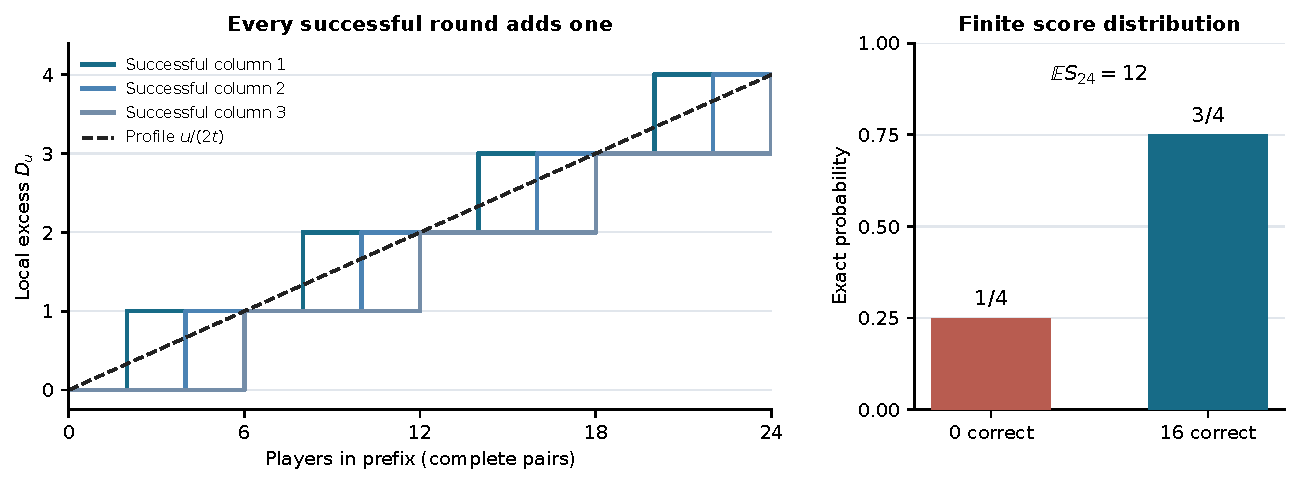
\includegraphics[width=\textwidth]{figures/02-hat-surplus-block_prefix.pdf}
\caption{Exact finite-block quantities for \(r=2,a=4\). The successful
even-prefix paths follow the line \(u/(2t)\) with uniformly bounded
error. The score distribution includes a common failure outcome;
the expected score remains \(N/2\). These are exact formulas, not
Monte Carlo estimates.}
\label{mbg:hat:fig:prefix}
\end{figure}

\section{Concatenation and a deterministic growth profile}
\label{mbg:hat:sec:clock}

Choose positive integers \(r_k,a_k\) and put
\[
  t_k=2^{r_k}-1,\qquad L_k=2a_kt_k,\qquad
  N_0=0,\quad N_k=\sum_{j=1}^kL_j.
\]
Block \(k\) consists of players \(N_{k-1}+1,\ldots,N_k\).
Every player uses only hats in that block. Let \(B_k\) be its
zero-syndrome event and put
\[
  p_k=\Prb(B_k)=\frac1{t_k+1}=2^{-r_k}.
\]
The events \(B_k\) are independent, though their independence is not
needed for the first Borel--Cantelli argument.

Define a deterministic continuous piecewise-linear function \(F\) on
\([0,\infty)\) by
\[
  F(n)=\sum_{j<k}a_j+\frac{n-N_{k-1}}{2t_k}
  \quad\text{when }N_{k-1}\le n\le N_k.                     \tag{22.1}\label{mbg:hat:eq:profile}
\]
The endpoint formulas agree, and \(F(N_k)=\sum_{j\le k}a_j\).
When \(t_k\) is nondecreasing, \(F\) is increasing and concave.

\begin{theorem}[Bounded random error]\label{mbg:hat:thm:tracking}
Suppose \(\sum_k2^{-r_k}<\infty\). Define the nonnegative extended
random variable
\[
  C=\sum_{k=1}^\infty a_k(t_k+1)\ind_{B_k}.                 \tag{22.2}\label{mbg:hat:eq:debt}
\]
Then \(C<\infty\) almost surely, and after the final bad block,
simultaneously for every physical prefix \(n\),
\[
  |D_n-F(n)+C|\le\frac32.                                \tag{22.3}\label{mbg:hat:eq:tracking}
\]
At every block endpoint, without any qualification on bad blocks,
\[
  D_{N_K}=\sum_{k\le K}a_k
          -\sum_{k\le K}a_k(t_k+1)\ind_{B_k}.             \tag{22.4}\label{mbg:hat:eq:debt-exact}
\]
For every hat assignment and every \(n\), one also has
\[
  D_n\le F(n)+\frac32.                                   \tag{22.5}\label{mbg:hat:eq:universalupper}
\]
\end{theorem}
\begin{proof}
The block excess is \(a_k\) in the good case and \(-a_kt_k\) in the
bad case. Rewriting it as
\(a_k-a_k(t_k+1)\ind_{B_k}\) proves the endpoint identity.
Since \(\sum_k\Prb(B_k)<\infty\), only finitely many \(B_k\) occur
almost surely. Every corresponding summand is finite, so \(C\) is
finite on that event.

Consider a prefix in a good block after the last bad one. The
completed blocks contribute \(\sum_{j<k}a_j-C\).
Lemma~\ref{mbg:hat:lem:prefix} bounds the current contribution by its linear
profile within \(3/2\), proving \eqref{mbg:hat:eq:tracking}. For the universal
upper bound, the accumulated debt from completed bad blocks is
nonnegative. A current good block satisfies the prefix bound, and a
current bad block contributes \(-u/2\le u/(2t_k)\). This proves
\eqref{mbg:hat:eq:universalupper} for all assignments.
\end{proof}

\begin{corollary}[Density and divergence]\label{mbg:hat:cor:density}
Under the hypotheses of Theorem~\ref{mbg:hat:thm:tracking}, assume also
\(t_k\to\infty\). Then
\[
  D_n\to+\infty,\qquad \frac{D_n}{n}\to0,\qquad
  \frac{S_n}{n}\to\frac12\quad\as.
\]
\end{corollary}
\begin{proof}
Since \(a_k\ge1\), \(F(N_k)\to\infty\); monotonicity gives
\(F(n)\to\infty\). To prove \(F(n)/n\to0\), fix \(\varepsilon>0\).
All sufficiently late slopes \(1/(2t_k)\) are at most
\(\varepsilon\), so \(F(n)\le A_\varepsilon+\varepsilon n\).
Divide by \(n\), let \(n\to\infty\), and then let
\(\varepsilon\downarrow0\). Theorem~\ref{mbg:hat:thm:tracking} now gives
the asserted almost-sure limits.
\end{proof}

\begin{proposition}[A quantitative stabilization bound]\label{mbg:hat:prop:confidence}
For any \(K\), with probability at least
\[
  1-\sum_{k\ge K}2^{-r_k},
\]
there are no bad blocks from \(K\) onward. On that event, every
\(n\ge N_{K-1}\) obeys
\[
  |D_n-F(n)|\le \sum_{j<K}a_j(t_j+1)+\frac32.
\]
For \(r_k=k\), the displayed failure bound is \(2^{1-K}\).
\end{proposition}
\begin{proof}
Use the union bound on \(\bigcup_{k\ge K}B_k\). The finite initial
debt is at most the displayed deterministic sum, and
\eqref{mbg:hat:eq:tracking} applies afterward.
\end{proof}

\subsection{Why this does not violate expectation}

For every finite \(n\), \(\E D_n=0\). Nevertheless the preceding
theorem gives \(D_n\to\infty\) almost surely. The exact accounting is
particularly transparent:
\[
  \E C
  =\sum_{k=1}^\infty a_k(t_k+1)\Prb(B_k)
  =\sum_{k=1}^\infty a_k
  =\infty.                                                \tag{22.6}\label{mbg:hat:eq:infinite-debt}
\]
Tonelli's theorem applies because the summands are nonnegative.
Thus the total debt is finite almost surely and has infinite
expectation. A rare failure of a sufficiently large block produces
a sufficiently large loss to maintain fairness at every finite
endpoint. An interchange of an almost-sure limit with expectation
would require an integrability hypothesis that is absent here.

\begin{writenote}[Added 4 October 2026, batch~90]
The divergence $D_n\to+\infty$ almost surely in Corollary~\ref{mbg:hat:cor:density} is not new as a phenomenon: Eldredge's Proposition~6.6~\cite{hat:Eldredge} already gives a measurable strategy with this property, built from independent blocks of growing length that follow the pairs strategy, except that a player who sees only black hats in its block guesses white; his blocks have a bad case (all hats black, every guess wrong), a good case adding one to the excess, and a neutral case, and the first and second Borel--Cantelli lemmas make bad blocks finitely many and good blocks infinitely many. His Remark~6.7 gives the explanation of this subsection: almost surely finitely many players sit in bad blocks, yet their expected number is infinite. What the syndrome blocks add is a gain proportional to the block length (Theorem~\ref{mbg:hat:thm:block-law}), the bound at every prefix (Lemma~\ref{mbg:hat:lem:prefix}) and hence the deterministic profile with bounded random error of Theorem~\ref{mbg:hat:thm:tracking}. The manuscript cites Eldredge's Proposition~6.6 only in its bibliography entry.
\end{writenote}

\section{An exact logarithmic answer and explicit faster examples}
\label{mbg:hat:sec:examples}

\begin{theorem}[Logarithmic excess]\label{mbg:hat:thm:log}
There is a computable finite-information compulsory strategy such that
\[
  D_n=\log_2 n+O_\omega(1)\quad\as.                       \tag{23.1}\label{mbg:hat:eq:log}
\]
Here \(O_\omega(1)\) means a finite bound depending on the hat
assignment, valid for every sufficiently large \(n\).
\end{theorem}
\begin{proof}
Take \(r_k=k\) and \(a_k=1\). Then
\[
  N_K=2\sum_{k=1}^K(2^k-1)=2^{K+2}-2K-4.
\]
For \(N_{k-1}<n\le N_k\), the profile \(F(n)\) lies between
\(k-1\) and \(k\). On the same interval,
\(\log_2 n=k+O(1)\), uniformly as \(k\to\infty\), since its
endpoints are bounded positive multiples of \(2^k\).
Therefore \(F(n)=\log_2 n+O(1)\). Summability of \(2^{-k}\) and
Theorem~\ref{mbg:hat:thm:tracking} prove \eqref{mbg:hat:eq:log}. All block
boundaries and finite rules are computable.
\end{proof}

This answers the logarithmic alternative itself, rather than only
providing a rate larger than a logarithm.

\begin{writenote}[Added 4 October 2026, batch~90]
Eldredge's first question in Remark~6.8~\cite{hat:Eldredge} (text checked at the write; Section~\ref{mbg:hat:sec:provenance}) asks for a measurable strategy whose excess $S_n-n/2$ is of order $\log n$ almost surely, in his sense of random constants $0<K_1<K_2<\infty$ and a random $N_0$ with $K_1\log\log n\le S_n-n/2\le K_2\log\log n$ for $n\ge N_0$ (stated there for $\log\log n$), ``or even some faster rate''. Theorem~\ref{mbg:hat:thm:log} gives more than order $\log n$: $D_n/\log_2 n\to1$ almost surely. Its strategy is continuous, hence measurable. Propositions~\ref{mbg:hat:prop:powers} and~\ref{mbg:hat:prop:nlogn} and Theorem~\ref{mbg:hat:thm:main} give the faster rates. Eldredge's own block strategy reaches orders $\log\log n$ and $\log n/(\log\log n)^2$ (his Remark~6.8).
\end{writenote}

\begin{proposition}[Every fixed power below one]\label{mbg:hat:prop:powers}
For every \(0<\beta<1\), a finite-information strategy satisfies
\[
  D_n\asymp n^\beta\quad\as,
\]
where the comparison holds for all sufficiently large \(n\).
For computable \(\beta\), one can use a computable schedule.
\end{proposition}
\begin{proof}
Take \(r_k=k\) and
\[
  a_k=\left\lceil2^{\beta k/(1-\beta)}\right\rceil.
\]
Geometric-sum estimates give
\[
  \sum_{j\le k}a_j\asymp2^{\beta k/(1-\beta)},\qquad
  N_k\asymp2^{k/(1-\beta)}.
\]
The implicit constants depend only on \(\beta\).
For a prefix in block \(k\), its index lies between endpoints
whose ratio is bounded, and its profile lies between consecutive
endpoint profiles whose ratio is also bounded.
Consequently \(F(n)\asymp n^\beta\) at every prefix.
Equation~\eqref{mbg:hat:eq:tracking} transfers this to \(D_n\).

For the effective assertion one may avoid exact ceiling decisions at
computable-real integer boundaries by choosing any effectively
computable integer approximation within a fixed factor of the
displayed \(a_k\). Such approximations preserve all estimates.
\end{proof}

\begin{proposition}[A concrete nearly linear example]\label{mbg:hat:prop:nlogn}
There is a computable finite-information strategy with
\[
  D_n\asymp\frac{n}{\log n}\quad\as.
\]
\end{proposition}
\begin{proof}
Set \(r_k=k\), \(a_k=2^{2^k}\). Since the final term dominates
each of the relevant sums,
\[
  N_k\asymp 2^k2^{2^k},\qquad
  F(N_k)\asymp2^{2^k},\qquad
  \log N_k\asymp2^k.
\]
For \(N_{k-1}\le n\le N_k\), one has
\(\log n\asymp2^k\). Nondecreasing \(t_j\) gives
\[
  F(n)\ge\frac{n}{2t_k}\asymp\frac n{\log n}.
\]
For the reverse bound, write
\[
  F(n)=F(N_{k-1})+\frac{n-N_{k-1}}{2t_k}.
\]
The first term is \(O(N_{k-1}/\log N_{k-1})\), which is
\(O(n/\log n)\) by eventual monotonicity of \(x/\log x\).
The second has that bound by \(\log n\asymp2^k\).
Apply \eqref{mbg:hat:eq:tracking}.
\end{proof}

These examples are mathematical constructions, not low-resource
algorithms. The number of visible hats used by a late player can
be very large. The general theorem next shows that no fixed
sublinear scale exhausts what is possible.

\section{No deterministic sublinear universal bound}
\label{mbg:hat:sec:main}

\begin{theorem}[Arbitrary prescribed sublinear growth]\label{mbg:hat:thm:main}
Let \(g:\N_{>0}\to(0,\infty)\) satisfy \(g(n)/n\to0\).
There is a finite-information continuous compulsory strategy such that
\[
  \frac{D_n}{g(n)}\longrightarrow+\infty
  \quad\text{and}\quad
  \frac{D_n}{n}\longrightarrow0
  \quad\as.                                               \tag{24.1}\label{mbg:hat:eq:main}
\]
The strategy can be chosen so that its excess tracks an increasing,
concave, deterministic function \(F=o(n)\) within a finite random
additive constant.
\end{theorem}
\begin{proof}
Put \(h(n)=\max\{g(n),\sqrt n\}\). Then \(h=o(n)\),
\(h(n)\to\infty\), and \(h\ge g\).
Fix \(r_k=k\) and \(t_k=2^k-1\).
For each \(k\ge2\), choose an integer \(R_k\) such that
\[
  n\ge R_k
  \quad\Longrightarrow\quad
  \frac{h(n)}{n}\le\frac1{k^2t_k}.                        \tag{24.2}\label{mbg:hat:eq:threshold}
\]
Such an integer exists by sublinearity. A least suitable integer
can be used, so no arbitrary selection among unrelated objects
is necessary.

Choose \(a_k\) recursively, always finite and positive, so that
\[
  N_k=N_{k-1}+2a_kt_k\ge R_{k+1}.                        \tag{24.3}\label{mbg:hat:eq:schedule}
\]
For example, once the thresholds are fixed, take the maximum of
\(1\) and the ceiling of
\((R_{k+1}-N_{k-1})/(2t_k)\).
The resulting disjoint blocks define one strategy before any hats
are sampled.

Consider an assignment with only finitely many bad blocks, and let
\(C\) be its finite debt. For \(n\) in a later good block \(k\),
monotonicity \(t_j\le t_k\) gives
\[
  F(n)
  =\sum_{j<k}\frac{L_j}{2t_j}
      +\frac{n-N_{k-1}}{2t_k}
  \ge\frac n{2t_k}.
\]
Using \eqref{mbg:hat:eq:tracking}, \eqref{mbg:hat:eq:threshold}, and
\(n\ge N_{k-1}\ge R_k\), we obtain
\[
  \frac{D_n}{h(n)}
  \ge
  \frac{n}{2t_kh(n)}-\frac{C+3/2}{h(n)}
  \ge \frac{k^2}{2}-\frac{C+3/2}{h(n)}.                  \tag{24.4}\label{mbg:hat:eq:main-estimate}
\]
Every block is finite, so \(k\to\infty\) with \(n\).
Since \(h(n)\to\infty\), the right side tends to infinity.
Thus \(D_n\) is eventually positive and
\(D_n/g(n)\ge D_n/h(n)\to\infty\).

The probability of finitely many bad blocks is one, since
\(\sum_k2^{-k}<\infty\). Finally \(F\) is increasing and concave
with slopes tending to zero, so \(F=o(n)\).
Theorem~\ref{mbg:hat:thm:tracking} proves the second limit and the tracking
assertion.
\end{proof}

\begin{corollary}[Failure of every proposed sublinear envelope]
\label{mbg:hat:cor:no-envelope}
There is no positive deterministic \(g=o(n)\) such that every
measurable legal strategy satisfies
\[
  \liminf_{n\to\infty}\frac{D_n}{g(n)}\le0
  \quad\as.
\]
There is also no such \(g\) for a universal finite upper bound on
that lower limit. Both assertions remain false when the strategies
are restricted to continuous finite-information strategies with
\(S_n/n\to1/2\) almost surely.
\end{corollary}
\begin{proof}
For any proposed \(g\), Theorem~\ref{mbg:hat:thm:main} supplies a strategy
whose ratio tends to \(+\infty\).
\end{proof}

\begin{remark}[Quantifier order]
The theorem says
\[
  \forall g=o(n)\quad \exists\text{ a strategy depending on }g.
\]
It does not say there is one strategy that dominates every
sublinear function. Indeed our fixed strategy tracks its own
deterministic \(F=o(n)\), and \(D_n/F(n)\to1\), so taking
\(g=F\) prevents that stronger statement.
\end{remark}

\begin{remark}[The wording of the published second question]\label{mbg:hat:rem:wording}
Eldredge's Remark~6.8 writes a universal equality for a normalized
lower limit. Its cited density theorem gives a nonpositive lower
limit, rather than equality for every strategy. Corollary
\ref{mbg:hat:cor:no-envelope} addresses the stronger meaningful obstruction:
even among strategies with eventually positive excess and limiting
success density \(1/2\), every prescribed sublinear scale fails.
Thus the equality wording does not affect the negative answer.
\end{remark}

\begin{writenote}[Added 4 October 2026, batch~90]
Checked against the text of v2~\cite{hat:Eldredge}. The source audit (\texttt{02-hat-surplus-\allowbreak source\_\allowbreak audit.txt}, item~1) says that Eldredge's Theorem~4.1 gives $\liminf D_n/n\le0\le\limsup D_n/n$, not equality for every measurable strategy. That is accurate, and Theorem~4.1 itself is not at fault: it is the density statement $L\le\frac12\le U$, which is \eqref{mbg:hat:eq:linear}, because $D_n/n=S_n/n-\frac12$. The wording issue is in the second question of Remark~6.8, which asks for $g$ with $\liminf_n(S_n-n/2)/g(n)=0$ almost surely for \emph{every} measurable strategy and says that Theorem~4.1 shows this for $g(n)=n$. Theorem~4.1 gives only ``$\le0$'', and equality does fail for some strategies. The write checked one, using this Part's blocks: take every $r_k=1$ (so each block of $a_k$ pairs is all right or all wrong, each with probability $1/2$, independently) and the dominant-block condition $L_k\ge kN_{k-1}$ of \eqref{mbg:hat:eq:dominance}. By the second Borel--Cantelli lemma infinitely many blocks are bad almost surely; at a bad endpoint $D_{N_k}/N_k\le1/(k+1)-1/2$, as in the proof of Theorem~\ref{mbg:hat:thm:category}, while $D_n/n\ge-1/2$ always; so $\liminf_nD_n/n=-1/2$ almost surely. This is a check made at the write, not a statement of the manuscript. Under the meaningful reading ``$\le0$'' Corollary~\ref{mbg:hat:cor:no-envelope} is the negative answer for every positive $g$ with $g(n)/n\to0$; under the literal reading the answer is negative a fortiori. Positive functions $g$ with $\limsup_n g(n)/n>0$ are outside the corollary's statement.
\end{writenote}

\section{The linear boundary remains unavoidable}
\label{mbg:hat:sec:linear}

For perspective, we give a short independent proof of the measurable
density obstruction, crediting the theorem to
\cite[Theorem~4.1]{hat:Eldredge}. The argument needs no assumptions about
the particular block construction.

\begin{theorem}[Measurable density obstruction]\label{mbg:hat:thm:linear}
For every measurable legal compulsory strategy,
\[
  \liminf_{n\to\infty}\frac{D_n}{n}\le0
  \le\limsup_{n\to\infty}\frac{D_n}{n}
  \quad\as.                                               \tag{25.1}\label{mbg:hat:eq:linear}
\]
In particular, no positive-probability event can support a strictly
positive asymptotic linear lower surplus.
\end{theorem}
\begin{proof}
Let \(T_i\) flip hat \(i\) and leave all other hats fixed.
The map preserves product probability. Put \(Y_i=Z_i-1/2\).
Legality implies \(Y_i\circ T_i=-Y_i\).

For any measurable event \(A\), invariance under \(T_i\) yields
\[
  \E[\ind_A Y_i]
  =\frac12\E[(\ind_A-\ind_A\circ T_i)Y_i],
\]
and hence
\[
  |\E[\ind_A Y_i]|\le\frac14\Prb(A\mathbin{\triangle}T_iA).
\]
The right side tends to zero. Indeed, approximate \(A\) in measure
by a finite-coordinate event \(A_0\). For all sufficiently large
\(i\), \(T_iA_0=A_0\), so
\(\Prb(A\triangle T_iA)\le2\Prb(A\triangle A_0)\).
Finite-coordinate events approximate all events in the completed
product sigma-field in measure.

Ces\`aro averaging now gives
\(\E[\ind_A D_n/n]\to0\). Apply this to
\(A=\{\liminf_n D_n/n>0\}\). Since \(D_n/n\) lies in
\([-1/2,1/2]\), Fatou's lemma applied after adding \(1/2\)
gives
\[
  \E\!\left[\ind_A\liminf_n\frac{D_n}{n}\right]\le0.
\]
Its integrand is strictly positive on \(A\), forcing \(\Prb(A)=0\).
Apply the same argument to \(-D_n\) for the second inequality.
\end{proof}

Theorems~\ref{mbg:hat:thm:main} and \ref{mbg:hat:thm:linear} give the exact
qualitative distinction relevant to the proposed envelope: linear
positive lower growth is impossible for measurable strategies,
while every fixed sublinear candidate can be defeated by a
continuous strategy.

\begin{writenote}[Added 4 October 2026, batch~90]
Theorem~\ref{mbg:hat:thm:linear} is Eldredge's Theorem~4.1~\cite{hat:Eldredge} restated for the surplus, as the manuscript says; it is inherited, not new. Eldredge requires each guess to be $\mu$-measurable (almost everywhere equal to a Borel function) and bases his proof on the martingale convergence of $\E[X\mid\mathcal F_m]$ (his Theorem~4.2); the proof above, by flip invariance and finite-coordinate approximation, is a second route to the same statement.
\end{writenote}

\section{Probability, Baire category, and the exact success set}
\label{mbg:hat:sec:category}

The preceding almost-sure behavior does not imply that the same
behavior is typical in the sense of Baire category. We can arrange
an explicit separation while retaining arbitrary prescribed growth.

In the construction of Theorem~\ref{mbg:hat:thm:main}, impose the additional
requirement
\[
  L_k=2a_kt_k\ge kN_{k-1}.                               \tag{26.1}\label{mbg:hat:eq:dominance}
\]
Increasing \(a_k\) can enforce this simultaneously with
\eqref{mbg:hat:eq:schedule}. Call this a \emph{dominant-block schedule}.

\begin{theorem}[Category behavior]\label{mbg:hat:thm:category}
For the dominant-block strategy associated to any positive \(g=o(n)\),
the following hold:
\begin{enumerate}
\item Almost surely \(D_n/g(n)\to+\infty\) and \(S_n/n\to1/2\).
\item For every hat assignment, \(\limsup_n S_n/n\le1/2\).
\item On a comeager subset of Cantor space,
\[
  \liminf_n\frac{S_n}{n}=0,\qquad
  \limsup_n\frac{S_n}{n}=\frac12.
\]
\end{enumerate}
\end{theorem}
\begin{proof}
The first conclusion is Theorem~\ref{mbg:hat:thm:main}.
The second follows from \eqref{mbg:hat:eq:universalupper} and \(F(n)/n\to0\).
For the third, note that every \(B_k\) is a nonempty clopen
finite-coordinate event, as is its complement. Because the blocks
are disjoint, each of
\[
  \bigcap_K\bigcup_{k\ge K}B_k,
  \qquad
  \bigcap_K\bigcup_{k\ge K}B_k^c
\]
is a dense \(G_\delta\): any finite prescription can be extended
to either type of pattern in a sufficiently late block.

At a bad block endpoint, all new guesses are wrong, so
\[
  \frac{S_{N_k}}{N_k}
  \le\frac{N_{k-1}}{N_{k-1}+L_k}\le\frac1{k+1}.
\]
At a good block endpoint, at least \(L_k/2\) new guesses are
correct, so
\[
  \frac{S_{N_k}}{N_k}
  \ge\frac{L_k/2}{N_{k-1}+L_k}\ge\frac{k}{2(k+1)}.
\]
On the comeager intersection of the two displayed sets, both kinds
of endpoints occur infinitely often. Nonnegativity of \(S_n\)
and the universal upper limit bound give the claimed limits.
\end{proof}

\begin{theorem}[Exact topological complexity]\label{mbg:hat:thm:success}
For the same dominant-block strategy, let
\[
  \mathcal S_g=\{\omega:D_n(\omega)/g(n)\to+\infty\}.
\]
Then
\[
  \mathcal S_g
  =\{\text{only finitely many }B_k\text{ occur}\}
  =\{\omega:S_n(\omega)/n\to1/2\}.                        \tag{26.2}\label{mbg:hat:eq:success}
\]
This set is dense, conull, meager, and
\(\boldsymbol{\Sigma}^0_2\)-complete under continuous reductions.
\end{theorem}
\begin{proof}
If only finitely many \(B_k\) occur, the deterministic proof of
Theorem~\ref{mbg:hat:thm:main} applies. If infinitely many occur,
the bad endpoints satisfy
\[
  \frac{D_{N_k}}{N_k}\le\frac1{k+1}-\frac12.
\]
Since \(g(N_k)/N_k\to0\), the ratio \(D_{N_k}/g(N_k)\)
tends to \(-\infty\) along those endpoints. Their success densities
also tend to zero. This proves both equalities in
\eqref{mbg:hat:eq:success}.

The event can be written as
\[
  \mathcal S_g=\bigcup_K\bigcap_{k\ge K}B_k^c.
\]
Each inner intersection is closed with empty interior, and therefore
nowhere dense. The union is \(F_\sigma\) and meager. It is dense
because any finite prescription can be extended to good patterns
in all sufficiently late blocks. It is conull by the first
Borel--Cantelli lemma.

For completeness, choose in every block a fixed bad pattern
(all hats zero) and a fixed good pattern (exactly one white hat
in its first pair). Given \(z\in\{0,1\}^{\N_{>0}}\), use the bad
pattern in block \(k\) if \(z_k=1\), and the good one if \(z_k=0\).
This defines a continuous map \(\Psi\), and
\[
  \Psi^{-1}(\mathcal S_g)
  =\FIN:=\{z:z_k=1\text{ for only finitely many }k\}.
\]
The set \(\FIN\) is
\(\boldsymbol{\Sigma}^0_2\)-complete; a self-contained verification
is given in Appendix~\ref{mbg:hat:app:fin}. Thus \(\mathcal S_g\) has the
claimed complexity.
\end{proof}

The completeness statement is topological, or boldface. With an
arbitrary \(g\), the block schedule need not be computable, so no
unqualified lightface complexity statement is being made.
The exact logarithmic schedule of Theorem~\ref{mbg:hat:thm:log} is a
different schedule and is not asserted to satisfy
\eqref{mbg:hat:eq:dominance}.

\section{Effective construction and finite information costs}
\label{mbg:hat:sec:effective}

\subsection{A computable schedule from a sublinearity modulus}

Suppose a function \(g\) is supplied with a computable modulus
\(M\) satisfying
\[
  n\ge M(b)\quad\Longrightarrow\quad
  g(n)/n\le2^{-b}.
\]
One can compute thresholds in \eqref{mbg:hat:eq:threshold}.
Choose \(b_k\) with \(2^{-b_k}\le1/(k^2t_k)\), and take
\[
  R_k=\max\{M(b_k),(k^2t_k)^2\}.
\]
Then both \(g(n)/n\) and \(1/\sqrt n\) satisfy the required bound.
Taking integer ceilings in \eqref{mbg:hat:eq:schedule}, and increasing
them if \eqref{mbg:hat:eq:dominance} is desired, gives a computable
sequence of finite blocks.

Given a player index, enumerate these increasing endpoints until
its block is located. The block has finitely many hats, and the
own-hat-excluding query set is computable. Thus the strategy is
a total truth-table procedure with a computable, but generally
unbounded, query bound.

An arbitrary computable function known abstractly to be \(o(n)\)
need not be accompanied by a computable convergence modulus.
The theorem without that extra information remains an existence
theorem for continuous strategies; it does not silently provide
uniform effective threshold selection.

\subsection{Algorithmically random assignments}

\begin{proposition}[An effective almost-sure refinement]
\label{mbg:hat:prop:mlrandom}
For a computable block schedule with \(r_k=k\), every Martin-L\"of
random hat sequence has only finitely many bad blocks.
Consequently all deterministic conclusions proved on that event
hold on every such sequence.
\end{proposition}
\begin{proof}
The events \(B_k\) are uniformly computable clopen events with
\(\Prb(B_k)=2^{-k}\). The effectively open sets
\[
  U_m=\bigcup_{k\ge m+1}B_k
\]
satisfy \(\Prb(U_m)\le2^{-m}\). They form a Martin-L\"of test.
A sequence belonging to infinitely many \(B_k\) belongs to every
\(U_m\), so it fails this test. Martin-L\"of random sequences avoid
that intersection.
\end{proof}

This is an effective form of the particular summable-event argument,
not a new general result in algorithmic randomness. Its relationship
to the stronger computable-randomness treatment in \cite{hat:EMV}
is part of the prior-art connection.

\subsection{What the finite algorithms cost}

For a block of \(N=2at\) physical players, the simplest individual
implementation reads all \(N-1\) other hats. It XORs visible pair
parities weighted by \(r\)-bit columns and applies the local rule.
This costs \(O(Nr)\) elementary bit operations under a direct
implementation, with \(O(r)\) working storage beyond query indexing
and counters. There is no communication of a shared syndrome.

For a centralized verifier that already has the full hat assignment,
one can calculate group parities and the syndrome once and derive
all guesses efficiently. That is a testing optimization, not the
information available to a player. The independent verifier in this
package explicitly checks own-hat blindness as well as agreement
between a group-based and a directly visible-pair implementation.

The ability to make a block arbitrarily long at fixed failure
probability is responsible for the arbitrary-growth theorem.
It is also why that theorem does not supply an economical visibility
bound as a function of player index. Quantitative restrictions on
visibility constitute a separate research problem.

\section{Verification and a concrete route into ProveIt}
\label{mbg:hat:sec:verification}

\subsection{Executed finite checks}

The archive contains a Python standard-library verifier and its
generated data. The following table records the actual exhaustive
cases. Prefix errors are computed as exact rational numbers.

\begin{center}
\begin{tabular}{rrrrrr}
\toprule
\(r\)&\(a\)&\(t\)&Players \(N\)&Assignments&Maximum prefix error\\
\midrule
1&1&1&2&4&0\\
1&2&1&4&16&0\\
1&3&1&6&64&0\\
1&4&1&8&256&0\\
1&5&1&10&1,024&0\\
2&1&3&6&64&1\\
2&2&3&12&4,096&1\\
2&3&3&18&262,144&1\\
3&1&7&14&16,384&\(9/7\)\\
\midrule
\multicolumn{4}{r}{Total assignments}&284,052&\\
\bottomrule
\end{tabular}
\end{center}

The completed run checked:
\begin{itemize}
\item \(5{,}010{,}248\) individual predictions against an independently
implemented rule;
\item \(10{,}020{,}496\) own-hat toggles across the two implementations;
\item \(3{,}997{,}918\) prefixes of nonzero-syndrome assignments,
including empty prefixes;
\item the full syndrome distribution, exact endpoint score law,
individual correctness probabilities, mean surplus, and second moment.
\end{itemize}
The measured run time was approximately \(17.2\) seconds in the
execution environment. This timing is descriptive, not a performance
guarantee.

For every parameter pair, the exact second moment is
\[
  \E[D_N^2]
  =a^2\frac{t}{t+1}
      +a^2t^2\frac1{t+1}
  =a^2t.
\]
This additional check detects incorrect gain/loss normalization.
The data also include explicit good and bad examples and a complete
prefix path.

Finite enumeration can detect an erroneous strategy, a hidden
own-coordinate dependency, or a wrong prefix constant. It does not
prove the theorem for all \(r,a\), and it cannot establish an
almost-sure statement over infinitely many blocks. Those claims
are proved in Sections~\ref{mbg:hat:sec:block}--\ref{mbg:hat:sec:main}.

\begin{writenote}[Added 4 October 2026, batch~90]
In the collection the verifier and the figure script are shipped as \texttt{code/\allowbreak 02-hat-surplus-\allowbreak verify\_\allowbreak hat\_\allowbreak strategy.py} and \texttt{code/\allowbreak 02-hat-surplus-\allowbreak make\_\allowbreak figures.py}, with the delivered \texttt{code/\allowbreak 02-hat-surplus-\allowbreak README.txt}, \texttt{code/\allowbreak 02-hat-surplus-\allowbreak Makefile} and the code's permissive licence \texttt{code/\allowbreak 02-hat-surplus-\allowbreak LICENSE.txt}; the recorded outputs are \texttt{data/\allowbreak 02-hat-surplus-\allowbreak verification.json}, \texttt{data/\allowbreak 02-hat-surplus-\allowbreak examples.json} and \texttt{data/\allowbreak 02-hat-surplus-\allowbreak example\_\allowbreak prefix.csv}, and the figure \texttt{figures/\allowbreak 02-hat-surplus-\allowbreak block\_\allowbreak prefix.pdf} (with a PNG copy), all byte-identical to the delivery. Run in place, the verifier would write unprefixed \texttt{verification.json}, \texttt{examples.json} and \texttt{example\_\allowbreak prefix.csv} into this report's \texttt{data/}, and the figure script unprefixed \texttt{block\_\allowbreak prefix.pdf} and \texttt{.png} into \texttt{figures/}, so both are rerun on a scratch copy; the report's \texttt{README.md} gives the commands. The timing of about 17.2 seconds above is the delivered run's (Python 3.12.14). At the write (4 October 2026, Python 3.14.4 on Windows, on a copy) the verifier passed all nine cases, with the totals of the table and list above, in about 112 seconds on a loaded machine (37 seconds at placement); the regenerated \texttt{examples.json} and \texttt{example\_\allowbreak prefix.csv} equal the shipped ones (the first after stripping the CR bytes Windows text mode writes), and \texttt{verification.json} does too apart from its completion time, Python version and elapsed-time fields. At placement the figure script, run on a copy with Matplotlib 3.10.8, reproduced the PDF figure up to its creation date, and the PNG at the same size with different bytes.
\end{writenote}

\subsection{Formalization layers}

A proof-assistant development can be divided into four small layers.
The following are proposed interfaces, not claims that the files
already exist.

\begin{enumerate}
\item \textbf{Finite semantics.}
Represent a hat assignment as \(\operatorname{Fin}(N)\to\mathrm{Bool}\).
Define a strategy as a family of Boolean functions and own-hat
blindness by invariance under a coordinate flip. Define score and
twice the surplus as integers, avoiding fractions initially.

\item \textbf{Syndrome algebra and counting.}
Represent columns in \(\F_2^r\); prove the two visibility cases and
the neutral case. Prove that the syndrome map is surjective and
that all its fibers have the same cardinality. The exact block law
then reduces to finite sums and a count of active columns.

\item \textbf{Physical order and prefixes.}
Use the lexicographic finite order on
\(\operatorname{Fin}(a)\times\operatorname{Fin}(t)\times
\operatorname{Fin}(2)\). Prove the division-with-remainder formula
for completed pairs. This isolates the part where a proof about
endpoints could otherwise be mistaken for a proof about all prefixes.

\item \textbf{Infinite product probability and asymptotics.}
Construct the disjoint finite blocks in countable product space.
Apply the first Borel--Cantelli lemma, establish the exact finite
debt identity, and then prove deterministic tracking and the
threshold schedule. This layer can use a standard library of
measure and asymptotic results.
\end{enumerate}

The existing \repo\ finite-list interfaces can encode the parameter
tables, predictions, and prefix certificates. A bridge to an
executable checker would require a theorem showing that accepted
certificates imply the intended finite statements. Merely evaluating
a Boolean checker or translating a program to arithmetic would not
establish that bridge.

\subsection{A sensible order of formal work}

The shortest useful first target is the finite theorem with arbitrary
\(r,a\), including blindness and the score law. The second is the
prefix lemma. These two targets already validate the complete local
mechanism. The third is the general concatenation theorem; once
available, logarithmic and arbitrary-growth schedules become
deterministic corollaries.

This order preserves a clear trust boundary. No claim about an
unformalized probability argument is promoted to kernel-checked
status merely because a finite arithmetic component has been
verified.

\section{Further research questions}
\label{mbg:hat:sec:questions}

The following are proposed follow-up problems. They are not presented
as a list of universally recognized open problems, and their precise
literature status should be checked before claiming a new solution.
They are chosen to continue the explicit connections among
prediction, asymptotics, computability, and formal verification.

\begin{question}[Which deterministic profiles admit bounded random error?]
Characterize increasing concave \(H=o(n)\) for which a compulsory
finite-information strategy satisfies
\[
  D_n=H(n)+O_\omega(1)\quad\as.
\]
Our construction realizes profiles with slopes
\(1/(2(2^{r_k}-1))\), integral gains per block, and summable bad-block
probabilities. Determine whether these restrictions are artifacts
of the construction or reflect a genuine obstruction to bounded
additive error.
\end{question}

\begin{question}[Information cost versus guaranteed growth]
Suppose player \(i\) may inspect at most \(q(i)\) other hats.
What excess profiles remain attainable? In particular, determine
whether a uniform bound on \(q(i)\) permits \(D_n\to+\infty\)
almost surely. Distinguish a bound on the number of queries from
a bound on their distance in the player ordering.
\end{question}

\begin{question}[Polynomially bounded visibility]
For an explicit target such as \(D_n\asymp n/\log n\), seek the
smallest possible maximum queried index as a function of \(n\).
The current construction is computable but its large blocks
give weak quantitative use bounds. An efficient construction
would strengthen the computational content of the result.
\end{question}

\begin{question}[The complete finite-team optimization problem]\label{mbg:hat:q:finiteteam}
For arbitrary \(N\) and threshold \(s>N/2\), determine
\[
  \sup_{\text{legal strategies}}\Prb(S_N\ge s).
\]
Corollary~\ref{mbg:hat:cor:finite-optimal} settles
\((N,s)=(2a(2^r-1),a2^r)\). For the remaining parameters,
identify exactly when the first-moment bound is attainable.
This is the most direct continuation of \repo's finite-team question.
\end{question}

\begin{question}[Classify equality cases]
For the parameters in Corollary~\ref{mbg:hat:cor:finite-optimal}, equality in
the first-moment bound forces the score to be supported on
\(\{0,s\}\). Classify legal strategies with that distribution,
up to relabeling players and hat colors. Determine how much of
the syndrome geometry follows from extremality alone.
\end{question}

\begin{question}[More than two colors]
Develop an analogue of the compulsory pairing transformation for
\(q\) equiprobable colors. A neutral group can have exactly one
correct guess, but an active group has a different gain/loss
balance from the binary case. Determine whether every
positive \(o(n)\) scale can be dominated above the baseline \(n/q\)
by finite-information strategies.
\end{question}

\begin{question}[Nonuniform and dependent hats]
Which parts of the theorem survive unequal known marginal
probabilities, or specified dependencies? Individual fairness
and uniform syndrome counting would both need replacement.
A useful first target is an independent binary product with
biases uniformly separated from zero and one.
\end{question}

\begin{question}[Precise distribution of the random debt]
For the logarithmic schedule,
\[
  C=\sum_{k\ge1}2^k\ind_{B_k},\qquad
  \Prb(B_k)=2^{-k}.
\]
Determine sharp tail asymptotics and possible oscillations caused
by the dyadic weights. Extend this to regularly varying choices
of \(a_k\). The distinction between almost-sure finiteness and
infinite mean is already settled, but finer distributional
questions are not addressed here.
\end{question}

\begin{question}[Best finite-horizon confidence guarantees]
Optimize the visibility and block lengths needed to ensure a
specified lower surplus after a specified index with probability
at least \(1-\delta\). Proposition~\ref{mbg:hat:prop:confidence} supplies
a direct bound, but it may be far from optimal when the cost of
the finite initial debt is included.
\end{question}

\begin{question}[Which pairs of measure and category behavior occur?]
The dominant-block construction is successful on a conull meager
set and has residual lower density zero. Characterize the
possible Borel complexities and residual density spectra of
continuous strategies with prescribed almost-sure excess growth.
Can similarly strong growth be arranged on a set that is both
conull and comeager?
\end{question}

\begin{question}[Effective randomness beyond the present test]
Determine the weakest standard randomness notion sufficient for
every computable schedule in this family. Compare that answer
with the computable-randomness results of \cite{hat:EMV}, taking care
to distinguish a fixed strategy with finitely many errors from
a sequence-dependent error-free autoreduction.
\end{question}

\begin{question}[A complete formal certificate chain]
Implement the four layers in Section~\ref{mbg:hat:sec:verification},
including a proved correspondence between an executable finite
checker and the mathematical semantics. Then formalize both
the rate theorem and the measure/category separation without
introducing an unproved probability or asymptotic axiom.
\end{question}

\subsection{Suggested priorities}

The best immediate formal target is the arbitrary-parameter finite
block theorem and prefix count. The best finite experimental target
is the optimization problem outside the dyadic family. The most
substantial structural targets are profile realization and
information-cost lower bounds. These directions ask for results
not supplied merely by repeating the arbitrary-growth scheduling
argument.

\begin{writenote}[Status of the questions, 4 October 2026, batch~90]
All twelve Research questions of this section stay open as printed; the intake searched no literature for them. Research question~\ref{mbg:hat:q:finiteteam} is the continuation, for fixed targets and binary hats, of Part~\ref{mbg:part:one}'s Q9, which Corollary~\ref{mbg:hat:cor:finite-optimal} settles for one family (see the note after the questions of Section~\ref{mbg:sec:questions}). Research question~29.6, on more than two colours, meets Part~\ref{mbg:part:one}'s $q$-ary setting; Research question~29.12 and the formalization layers above are proposals, and no Lean or Rocq file of ProveIt implements any of them.
\end{writenote}


% Part II's appendices continue Part I's letters.
\setcounter{section}{2}
\renewcommand{\thesection}{\Alph{section}}
\renewcommand{\theHsection}{hat.app.\Alph{section}}
\makeatletter\gdef\Hy@chapapp{\Hy@appendixstring}\makeatother

\section{The exact prefix constant}
\label{mbg:hat:app:prefix}

The convenient bound \(3/2\) in Lemma~\ref{mbg:hat:lem:prefix} can be
replaced by an optimal parameter-dependent constant.

\begin{proposition}\label{mbg:hat:prop:sharp-prefix}
For \(t=2^r-1\), the largest possible value of
\[
  \left|D^{\rm loc}_u-\frac{u}{2t}\right|
\]
over all nonzero-syndrome assignments and all prefixes in a block
with \(a\ge1\) is
\[
  B_t=\frac{3(t-1)}{2t}.
\]
\end{proposition}
\begin{proof}
For \(t=1\), every pair in a good block is fully correct, so the
error is zero. Assume \(t\ge3\).
At an even prefix with \(p=qt+j\) completed pairs,
the error is
\[
  e_{2p}=\ind_{\{c\le j\}}-\frac jt.
\]
Its absolute value is at most \((t-1)/t\).

At the next odd prefix, add
\(z-1/2-1/(2t)\), where \(z\) is the next player's correctness
indicator. There are three cases.
If \(j+1=c\), the next pair is active and \(z=1\); the
resulting absolute error is at most \((t-1)/(2t)\).
If \(j+1<c\), then \(j\le t-2\), the active pair is still ahead,
and using \(z\in\{0,1\}\) gives the lower bound
\[
  -\frac{t-2}{t}-\frac12-\frac1{2t}
  =-\frac{3(t-1)}{2t}.
\]
The corresponding upper bound is smaller.
If \(c\le j\), then \(j\ge1\), and the largest possible error is
\[
  1-\frac1t+\frac12-\frac1{2t}
  =\frac{3(t-1)}{2t}.
\]
The lower bound in that case is smaller in absolute value.
This proves the bound.

For attainment, set exactly one of the hats in the very first
column-\(1\) pair to one, and all other hats to zero.
Then \(\sigma=h_1\), and the first pair is fully correct.
The first player in the next, neutral pair also guesses correctly,
so \(D^{\rm loc}_3=3/2\). Its deviation from \(3/(2t)\) equals
\(B_t\).
\end{proof}

The exhaustive data attain \(B_1=0\), \(B_3=1\), and
\(B_7=9/7\), matching this general proof.

\section{A self-contained completeness fact for FIN}
\label{mbg:hat:app:fin}

We include the elementary descriptive-set-theoretic fact used in
Theorem~\ref{mbg:hat:thm:success}.

\begin{proposition}
The subset \(\FIN\) of Cantor space consisting of sequences with
finitely many ones is
\(\boldsymbol{\Sigma}^0_2\)-complete under continuous reductions
from Cantor space.
\end{proposition}
\begin{proof}
It is \(F_\sigma\), since
\[
  \FIN=\bigcup_m\bigcap_{n\ge m}\{z:z_n=0\}.
\]
Let \(A=\bigcup_j C_j\) be any \(F_\sigma\) subset of Cantor
space. By taking finite unions, assume the closed sets \(C_j\)
are increasing. For a point \(x\), and each stage \(n\), let
\(m_n(x)\) be the least \(j\le n\) such that the cylinder
determined by the first \(n\) bits of \(x\) meets \(C_j\);
if there is no such \(j\), put \(m_n(x)=n+1\).

Each \(m_n\) depends only on a finite prefix. Moreover
\(m_{n+1}(x)\ge m_n(x)\): shrinking a cylinder cannot make it
meet a previously excluded closed set, and a newly introduced
index is no smaller than the previous default.
Define a bit sequence \(z(x)\) by setting
\[
  z_n(x)=
  \begin{cases}
  1,&m_{n+1}(x)>m_n(x),\\
  0,&m_{n+1}(x)=m_n(x).
  \end{cases}
\]
This map is continuous.

If \(x\in C_J\), every cylinder around \(x\) meets \(C_J\).
Thus \(m_n(x)\le J\) for \(n\ge J\). Being nondecreasing,
the sequence \(m_n(x)\) is eventually constant, so \(z(x)\)
has finitely many ones.
If \(x\notin A\), then for each fixed \(J\), closedness of
\(C_J\) implies some sufficiently short neighborhood of \(x\)
misses it. Since the \(C_j\) are increasing,
\(m_n(x)>J\) for all sufficiently large \(n\).
Therefore \(m_n(x)\to\infty\) and changes infinitely often,
so \(z(x)\notin\FIN\). Hence \(z^{-1}(\FIN)=A\).
\end{proof}

\section{Reproducibility and source notes}
\label{mbg:hat:app:repro}

\subsection{Files and commands}

The package contains the complete LaTeX source, compiled PDF,
the finite verifier, exact JSON results, a CSV prefix example,
and the figure-generation script. Build commands are recorded
in \texttt{README.txt} and \texttt{Makefile}.

From the package directory:
\begin{lstlisting}
python3 code/verify_hat_strategy.py
python3 code/make_figures.py
pdflatex -interaction=nonstopmode -halt-on-error hat_guessing_growth.tex
pdflatex -interaction=nonstopmode -halt-on-error hat_guessing_growth.tex
pdflatex -interaction=nonstopmode -halt-on-error hat_guessing_growth.tex
\end{lstlisting}
The verifier needs only the Python standard library.
Regenerating the plots additionally needs Matplotlib.
The complete mathematical proofs are in the LaTeX source;
they do not depend on the image files.

\begin{writenote}[Added 4 October 2026, batch~90]
These commands and file names are the delivery's. In the collection the manuscript's source and PDF, \texttt{hat\_\allowbreak guessing\_\allowbreak growth.tex} and \texttt{.pdf}, and the delivered top-level \texttt{README.txt} are not shipped (this Part is the source, built as part of the report's \texttt{article.tex}); they survive in the archive of the arrival commit \texttt{a162e4386}. The shipped names are listed in the note of Section~\ref{mbg:hat:sec:verification}, and the delivered \texttt{code/\allowbreak 02-hat-surplus-\allowbreak Makefile} and \texttt{code/\allowbreak 02-hat-surplus-\allowbreak README.txt} still use the delivery names; the report's \texttt{README.md} gives reruns that work with the shipped names, on a scratch copy.
\end{writenote}

\subsection{Source distinctions}

The main literature checks used the primary arXiv text of
\cite{hat:Eldredge}, the official journal record and author-uploaded
final text of \cite{hat:EMV}, and the exact repository snapshot.
The older ECCC preprint is also listed for access.
Some hosting-page metadata describes an earlier conference
version of the autoreducibility paper; the final text itself
identifies the three authors, the 2003 SIAM publication, and
the DOI given below.

The key conclusion is a direct theorem with a complete proof.
The historical question of whether this exact compulsory-guess
formulation appeared elsewhere is separate, and remains unverified.
The report should be cited or circulated with that distinction
intact.

\clearpage
\fancyhead[R]{\small Research note}
\begin{thebibliography}{10}
\bibitem{GlazerBox}
Elliot Glazer, \emph{A choiceless box game paradox}, arXiv:2211.10474, submitted 2022; inspected PDF dated January 9, 2023. \url{https://arxiv.org/abs/2211.10474}.
{\small[write, 3 October 2026: arXiv lists one version, v1 of 15 November 2022, 6 pages, math.LO and math.CO, DOI \nolinkurl{10.48550/arXiv.2211.10474}; the date January 9, 2023 is printed in arXiv's PDF of v1.]}

\bibitem{GlazerChoice}
Elliot Glazer, \emph{Global choice is not conservative over local choice for Zermelo set theory}, arXiv:2312.11902. \url{https://arxiv.org/abs/2312.11902}.

\bibitem{GlazerProfile}
Tamay Besiroglu, Elliot Glazer, and Caroline Falkman Olsson,
\emph{FrontierMath competition: Setting benchmarks for AI evaluation}, January 16, 2025, updated March 18, 2025; author profile of Elliot Glazer.
\url{https://samaritan-research.org/blog/frontiermath-competition-setting-benchmarks-for-ai-evaluation}.

\bibitem{LosMarczewski}
J. \L o\'s and E. Marczewski, \emph{Extensions of measure}, Fundamenta Mathematicae \textbf{36} (1949), 267--276.
Catalog: \url{https://eudml.org/doc/213194}.
Inspected scan: \url{https://scispace.com/pdf/extensions-of-measure-v0jwsbilmx.pdf}.

\bibitem{OEIS}
The OEIS Foundation, \emph{A005271: Number of perfect matchings in $n$-cube}. \url{https://oeis.org/A005271}. Accessed October 3, 2026.

\bibitem{ProveIt}
Vladimir Reshetnikov, \emph{ProveIt}, repository snapshot \commit.
\url{https://github.com/VladimirReshetnikov/ProveIt}.

\bibitem{BusyBeaver}
\repo\ contributors, \emph{BusyBeaver/Core.lean}, at the snapshot in \cite{ProveIt}, particularly its introductory machine/maximum/compiler interface and coordinate read/write lemmas.
\url{https://github.com/VladimirReshetnikov/ProveIt/blob/6fef5383b126be343cccc9baf47081ef37ab5afe/Computability/BusyBeaver/Lean/BusyBeaver/Core.lean}.

\bibitem{ListCoding}
\repo\ contributors, \emph{Coding finite lists in Peano arithmetic}, project README at the snapshot in \cite{ProveIt}.
\url{https://github.com/VladimirReshetnikov/ProveIt/blob/6fef5383b126be343cccc9baf47081ef37ab5afe/Logic/PeanoArithmetic/ListCoding/README.md}.

\bibitem{Closure}
\repo\ contributors, \emph{Closure axiomatization of set theory}, project README at the snapshot in \cite{ProveIt}.
\url{https://github.com/VladimirReshetnikov/ProveIt/blob/6fef5383b126be343cccc9baf47081ef37ab5afe/SetTheory/ClosureAxiomatization/README.md}.

% Part II's entries (batch 90); its Glazer entry is GlazerBox above.
\raggedright
\bibitem{hat:Eldredge}
Nathaniel Eldredge.
\emph{A probabilistic look at the infinite hat-guessing game}.
arXiv:2508.02828v2, October 24, 2025.
\url{https://arxiv.org/html/2508.02828v2}.
DOI: \href{https://doi.org/10.48550/arXiv.2508.02828}
{10.48550/arXiv.2508.02828}.
See Theorem~4.1 and Proposition~6.6--Remark~6.8.
{\small[write, 4 October 2026: the arXiv record lists v1 of 4 August 2025 and v2 of 24 October 2025, 20 pages, math.PR with math.LO; the v2 text was read at the write (Section~\ref{mbg:hat:sec:provenance}).]}

\bibitem{hat:EMV}
Todd Ebert, Wolfgang Merkle, and Heribert Vollmer.
\emph{On the Autoreducibility of Random Sequences}.
SIAM Journal on Computing \textbf{32}(6) (2003), 1542--1569.
DOI: \href{https://doi.org/10.1137/S0097539702415317}
{10.1137/S0097539702415317}.
See especially Theorem~6.6 and its proof.
Preprint: \url{https://eccc.weizmann.ac.il/report/2002/056/}.
{\small[write, 4 October 2026: the ECCC record (TR02-056, 19 September 2002, same authors and title) was read; the SIAM text and its Theorem~6.6 were not checked at the write.]}

\bibitem{hat:ProveItBoxes}
Vladimir Reshetnikov, \repo\ repository.
\emph{Countable Information, Uncountably Many Boxes:
Sharp measurable prediction bounds, exact decision-tree
enumeration, and an all-orders asymptotic expansion}.
Research report dated October 3, 2026.
Inspected in repository commit
\texttt{7c0f2d9f92c3d51ec85703bed1022924a4b7359b}.
\url{https://github.com/VladimirReshetnikov/ProveIt}.
Path:
\texttt{SetTheory/Cardinals/docs/reports/ordinals-and-order-types/}
\texttt{measurable-box-games/article.tex}.
See the ninth further-research item.
{\small[write, 4 October 2026: this is Part~\ref{mbg:part:one} of the present report; the ninth item is its Research question~Q9.]}

\bibitem{hat:ProveItCoding}
Vladimir Reshetnikov, \repo\ repository.
\emph{Peano arithmetic finite-list coding}.
Same repository snapshot.
Path: \texttt{Logic/PeanoArithmetic/ListCoding/README.md},
with \texttt{PAListCoding/Basic.lean} and
\texttt{PAListCoding/Predicates.lean} under its Lean directory.
\url{https://github.com/VladimirReshetnikov/ProveIt}.
\end{thebibliography}
\end{document}
